\documentclass{beamer}
\usetheme{dianahep}

%
% Title definitions
%

\title{The DIANA/HEP and S2I2-HEP projects, \\
       the HEP Software Foundation \\
       and the Community White Paper \\
       Towards Sustainable Software}
\author{Peter Elmer - Princeton University}
\date{10 January, 2017 \\ JLab Computing Round Table}

\begin{document}
\maketitle
%\insertframenumber/\inserttotalframenumber

%
% Presentation body
%

\setbeamertemplate{footline}[frame number]

\begin{frame}
\frametitle{My background}

\begin{itemize}
\item I'm a staff scientist with Princeton University, based at CERN
\item In the past I've worked on the ALEPH experiment at CERN and the BaBar experiment at SLAC
\item I was heavily involved in Software and Computing in BaBar and since 2004 I've worked on Software and Computing in CMS in a variety of organizational roles. 
\item I'm also the PI for two NSF project (DIANA/HEP and S2I2-HEP) and involved with the HEP Software Foundation.
\end{itemize}

\end{frame}




\begin{frame}
\frametitle{Overview}

In this presentation I will talk about several things:

\begin{itemize}
\item Software Challenges and Sustainability for HEP in the 2020s
\item The DIANA/HEP project
\item The S2I2-HEP ``Software Institute'' conceptualization project
\item The HEP Software Foundation and the ``Community White Paper'' roadmap project
\end{itemize}

I'll also explain the ways in which these are related...

\end{frame}




\begin{frame}
\frametitle{CERN Accelerator Timeline}

\begin{figure}[htbp]
\begin{center}
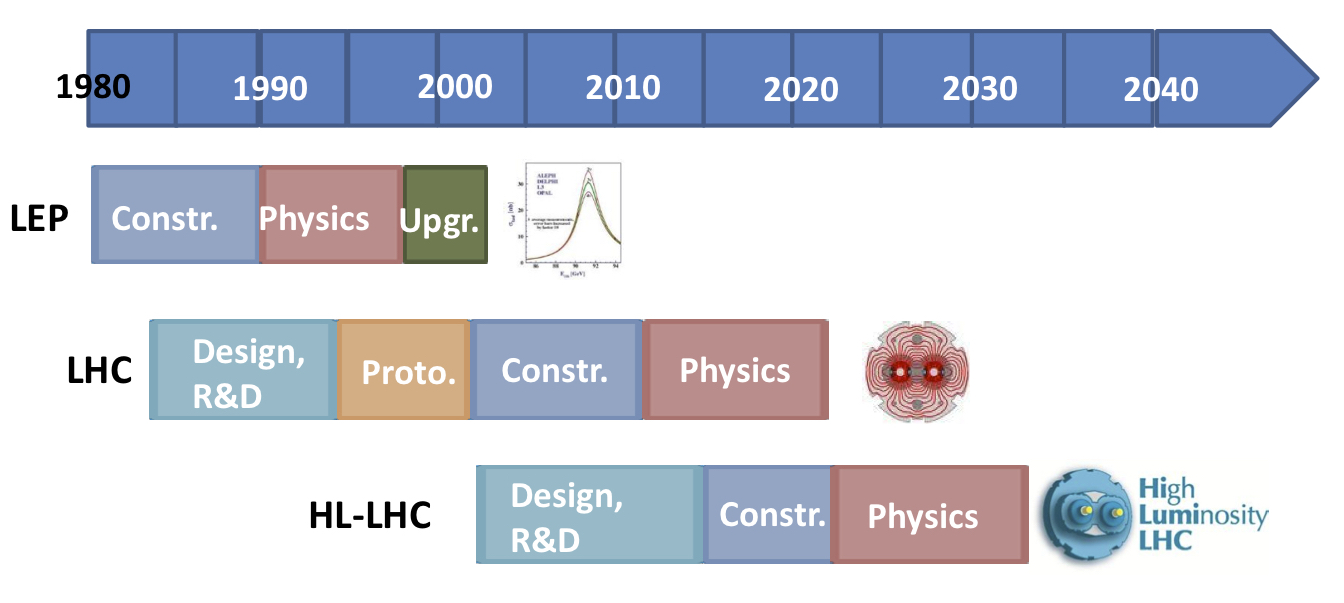
\includegraphics[width=1.0\textwidth]{images/timelineCERNprojects_image_current.jpg}
%\caption{}
%\label{fig:example2}
\end{center}
\end{figure}

\small{Various concepts also exist for subsequent machines.}

\end{frame}




\begin{frame}
\frametitle{Plans for upgrading the LHC and Experiment Detectors}

\begin{figure}[htbp]
\begin{center}
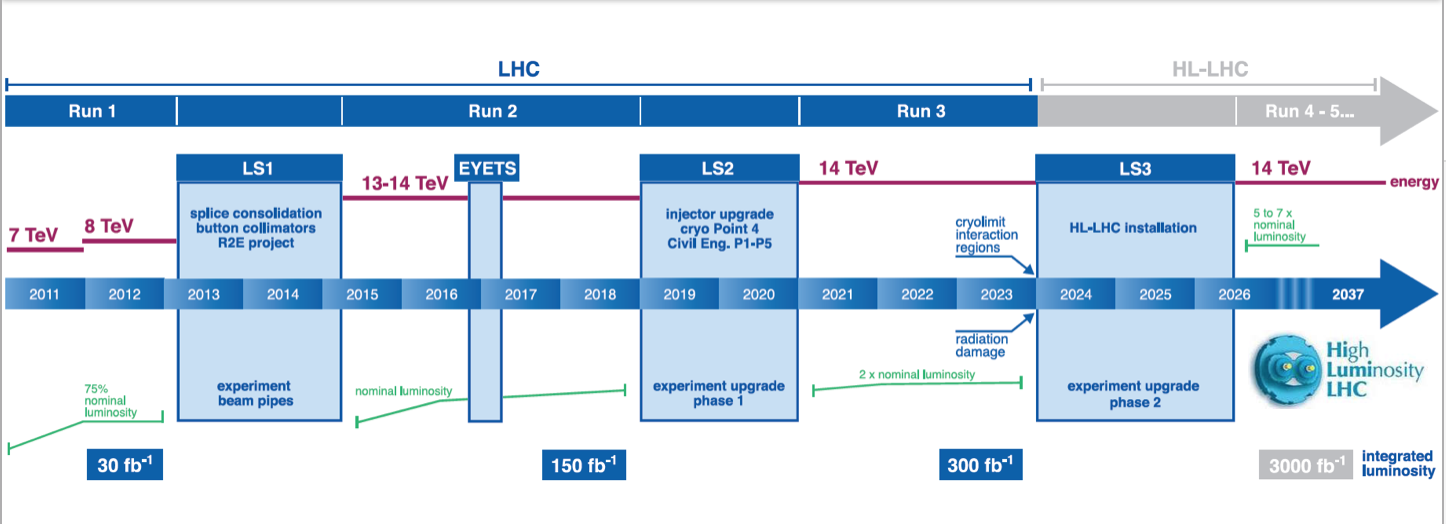
\includegraphics[width=1.0\textwidth]{images/lhc-upgrade-timeline-detail.png}
%\caption{}
%\label{fig:example2}
\end{center}
\end{figure}

%\small{Example Text}

\end{frame}



\begin{frame}
\frametitle{A Software ``Upgrade'' for HL-LHC and 2020s HEP?}

Looking forward to the next 10 years, we see a number of challenges for HEP software and computing:

\begin{itemize}
\item {\bf Scale:} The HL-LHC will integrate 100 times the current data, with significantly increased data (pileup) and detector complexity.
\item {\bf Performance/cost:} Estimates of computing needs run faster than Moore's Law by factors of 3-30
\item {\bf Technology/Market evolution:} the return of heterogeneity; technology change will also make it challenging to exploit Moore's Law without software evolution.
\item {\bf Sustainability:} Most of the current software, which defines our capabilities, was designed 15-20 years ago: there are many software sustainability challenges.
\end{itemize}

\end{frame}



\begin{frame}
\frametitle{Why Software? Software is {\em the} Cyberinfrastructure}

\begin{figure}[htbp]
\begin{center}
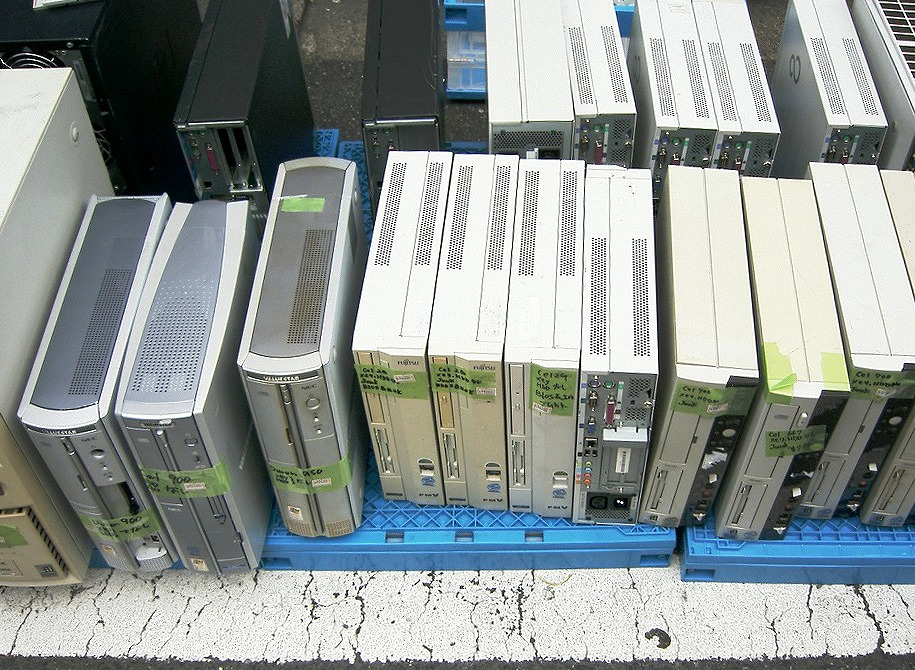
\includegraphics[width=0.7\textwidth]{images/Junk_desktop_personal_computer.jpg}
%\caption{}
%\label{fig:example2}
\end{center}
\end{figure}

\begin{center}
\small{Computer hardware is a consumable. \\ Software is what we keep, and invest in, over time.}
\end{center}

\end{frame}




\begin{frame}
\frametitle{Estimates of Resource Needs for HL-LHC (WLCG)}

\begin{figure}[htbp]
\begin{center}
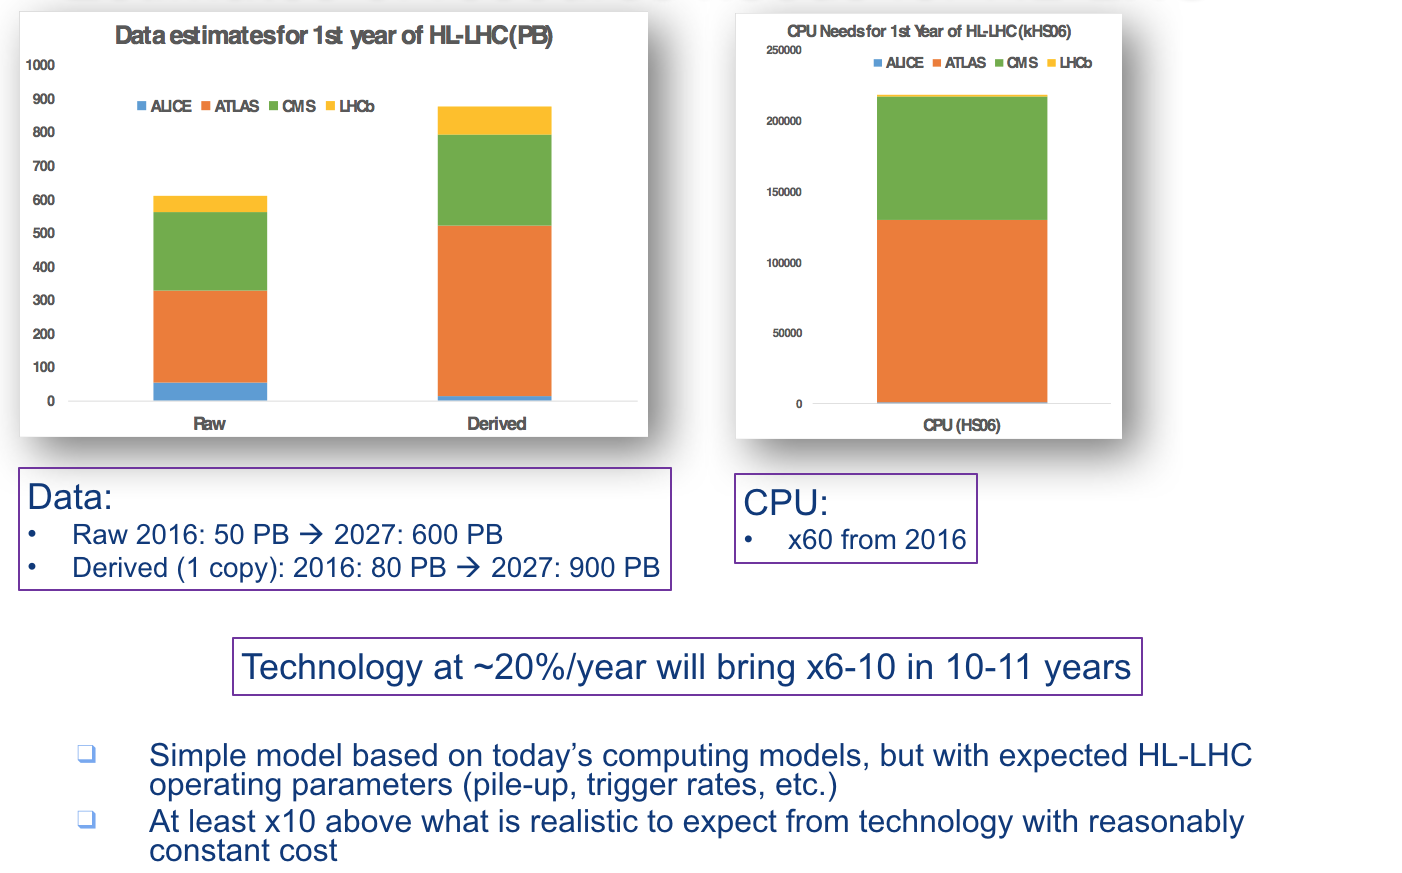
\includegraphics[width=0.9\textwidth]{images/20161008-wlcg-intro-ian-bird-slide-10.png}
\end{center}
\end{figure}

\begin{center}
\small{(Slide from WLCG Workshop Intro, Ian Bird, 8 Oct, 2016)}
\end{center}

\end{frame}




\begin{frame}
\frametitle{Processor evolution and software impact}

\begin{columns}[T] % align columns

\begin{column}{.48\textwidth}
\begin{figure}[htbp]
\begin{center}
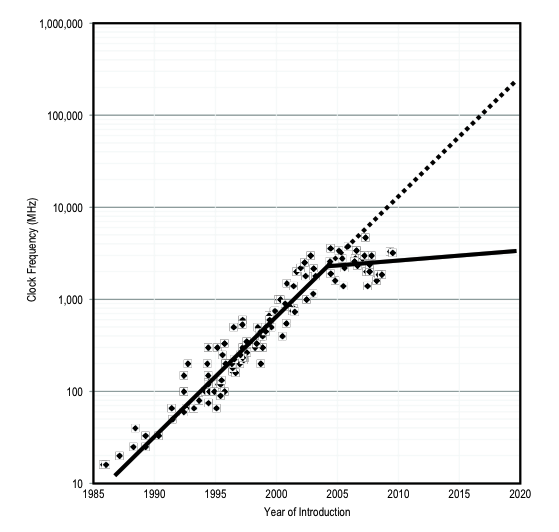
\includegraphics[width=1.0\textwidth]{images/moore2.png}
\end{center}
\end{figure}
\begin{center}
\small{Clock Frequency vs Time}
\end{center}
\end{column}%

\hfill%

\begin{column}{.48\textwidth}
\begin{itemize}
\item Single core performance has stalled, leading to multi/manycore and specialization
\item To even realize Moore's Law gains, we are pushed towards parallelization of algorithms and design for performance.
\item The software designs and implementations themselves need to evolve, not just be recompiled
\end{itemize}
\end{column}%

\end{columns}

\end{frame}



\begin{frame}
\frametitle{Back to heterogeneous systems?}

Building the worldwide distributed LHC computing grid was largely made possible by the convergence on Linux on (commodity) Intel x86 processors around the year 2000. Building the WLCG at this scale in the heterogeneous workstation era would have been quite difficult. For better or for worse, heterogeneity is returning:

\begin{itemize}
\item Diversity of computing processor architectures (general purpose cores vs specialized processors)
\item Owned vs commercial/cloud providers
\item Some pressure to use systems traditionally designed for other types of applications (e.g.\ HPC/supercomputer as opposed to HTC/high-throughput systems)
\item Possible further commoditizing market pressures (e.g. mobile)
\end{itemize}

\end{frame}




\begin{frame}
\frametitle{What is software sustainability?} 
\begin{itemize}
\item {\bf Dependent Infrastructure:} Will the infrastructure element continue to provide the same functionality in the future, even when the other parts of the infrastructure on which the element relies change?
\item {\bf Collaborative Infrastructure} Can the element be combined with other elements to meet user needs, as both the collaborative elements and the individual elements change?
\item {\bf New Users:} Is the functionality and usability of the infrastructure element clearly explained to new users? Do users have a mechanism to ask questions and to learn about the element?
\item {\bf Existing Users:} Does the infrastructure element provide the functionality that current users want? Is it modular and adaptable so that it can meet the future needs of the users?
\item {\bf Science:} Does it incorporate and implement new science and theory as they develop?
\end{itemize}

\tiny{ Katz, D.S. \& Proctor, D., (2014). A Framework for Discussing e-Research Infrastructure Sustainability. Journal of Open Research Software. 2(1), p.e13. DOI: http://doi.org/10.5334/jors.av}
\end{frame}



\begin{frame}
\frametitle{Likely constraints to fund a ``Software Upgrade''}

It appears unlikely that significant increases in investments in software 
will be made by funding agencies purely from particle physics budgets 
and/or into individual experiments. Other opportunities do perhaps exist,
but often imply constraints, for example:

\begin{itemize}
\item Investments into software impacting multiple experiments 
\item Investments into development with impact beyond particle physics 
\item Investments into development permitting use of computing facilities (e.g. HPC) planned for other non-HEP purposes
\item Investments requiring collaborations with Computer Science or Industry
\end{itemize}

Building the LHC software in use today was possible without too many such constraints. The good news is that the community (with an existing LHC computing system) is better positioned today to make effective progress even with such constraints.

\end{frame}


\begin{frame}
\frametitle{HEP Software Ecosystem}

\begin{figure}[htbp]
\begin{center}
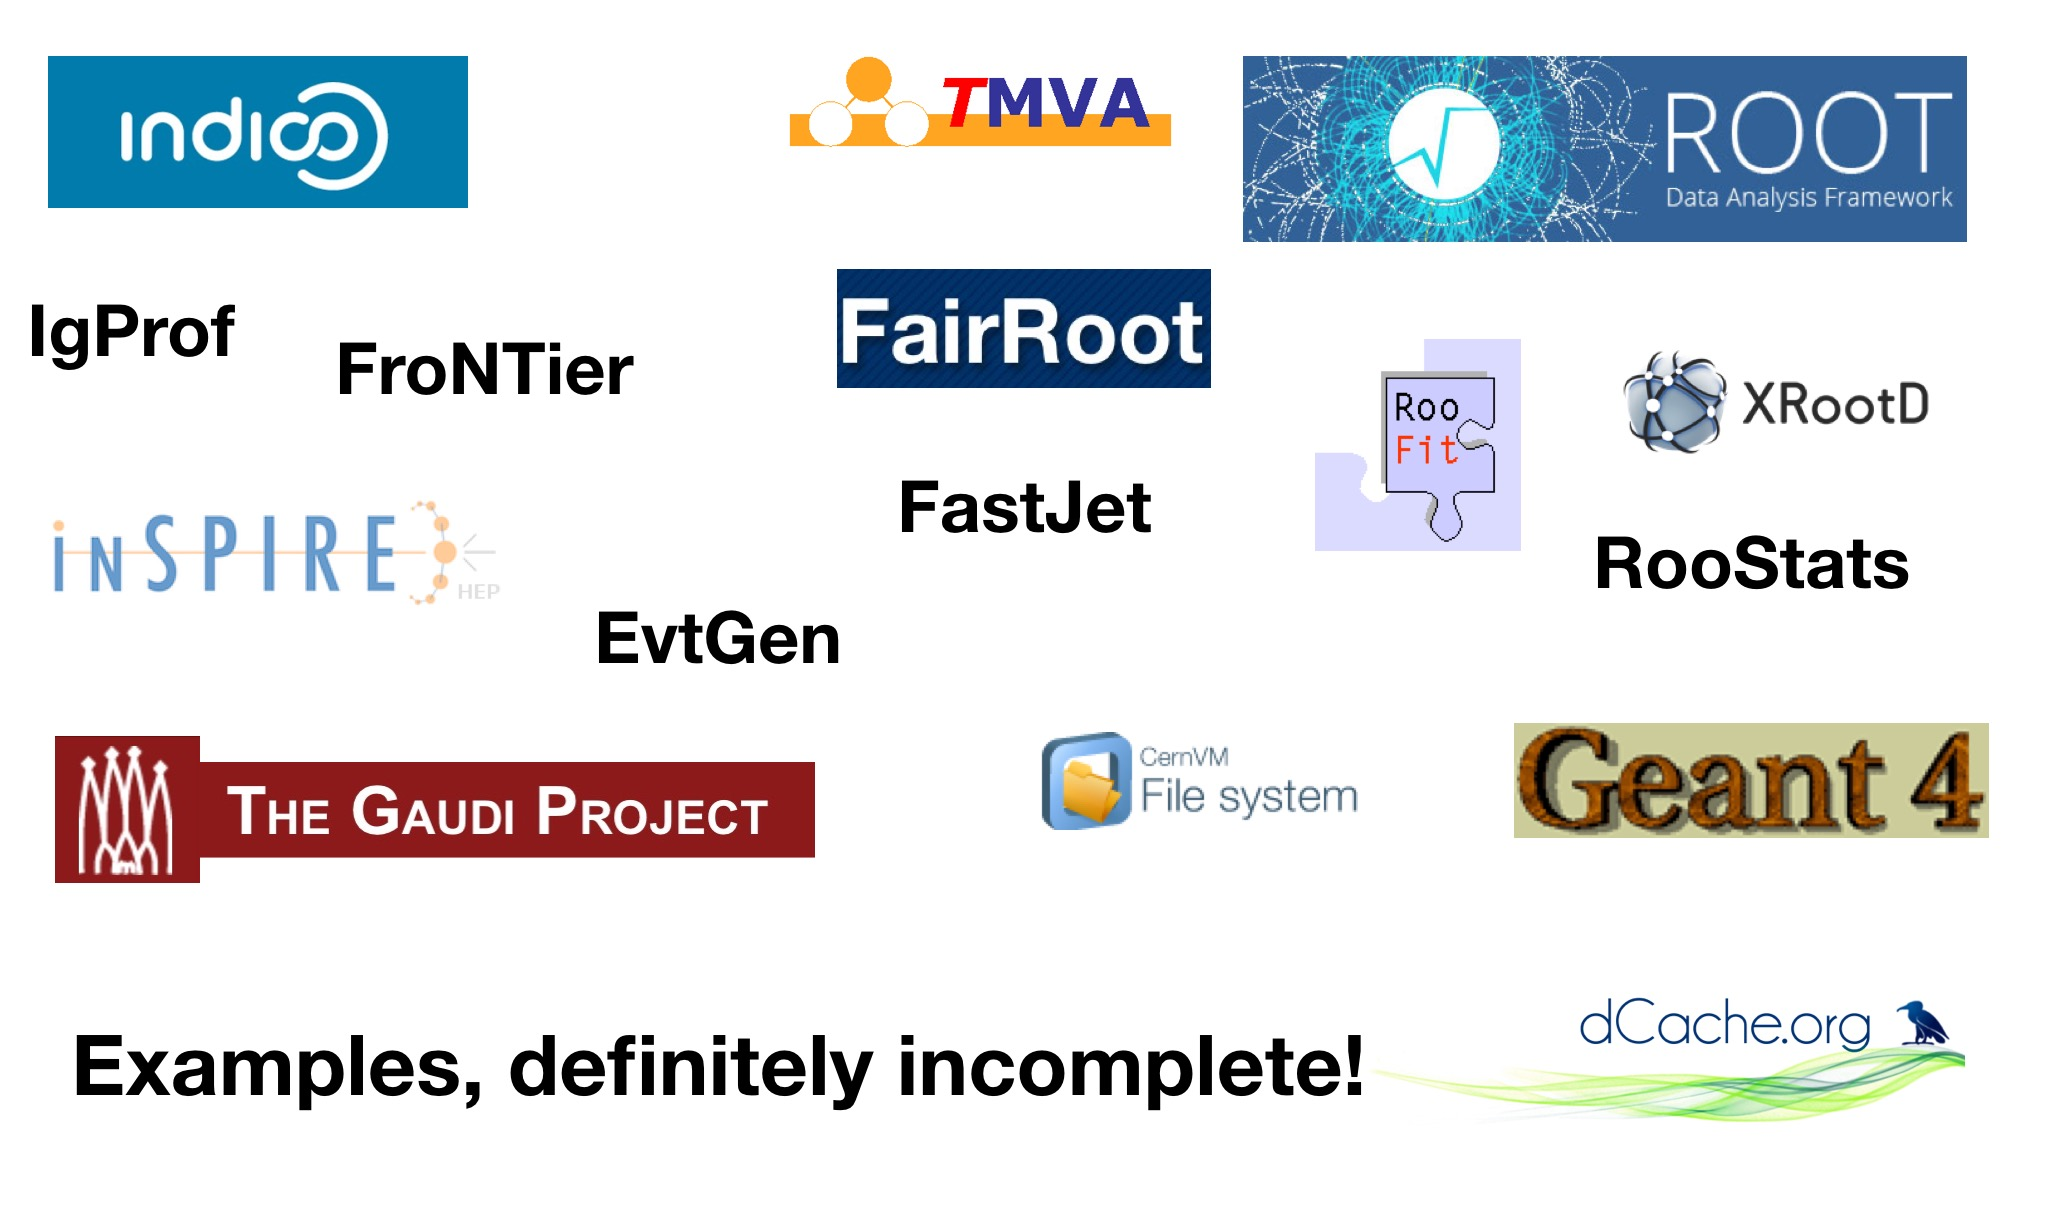
\includegraphics[width=0.9\textwidth]{images/hep-software-ecosystem.jpg}
\end{center}
\end{figure}

{\small Plus 15-20M Source Lines of Code (SLOC) of ``experiment specific'' codes, as well as dependencies on non-HEP scientific software.}
\end{frame}




\begin{frame}
\frametitle{Software Infrastructure for Sustained Innovation (SI2)}

\begin{figure}[htbp]
\begin{center}
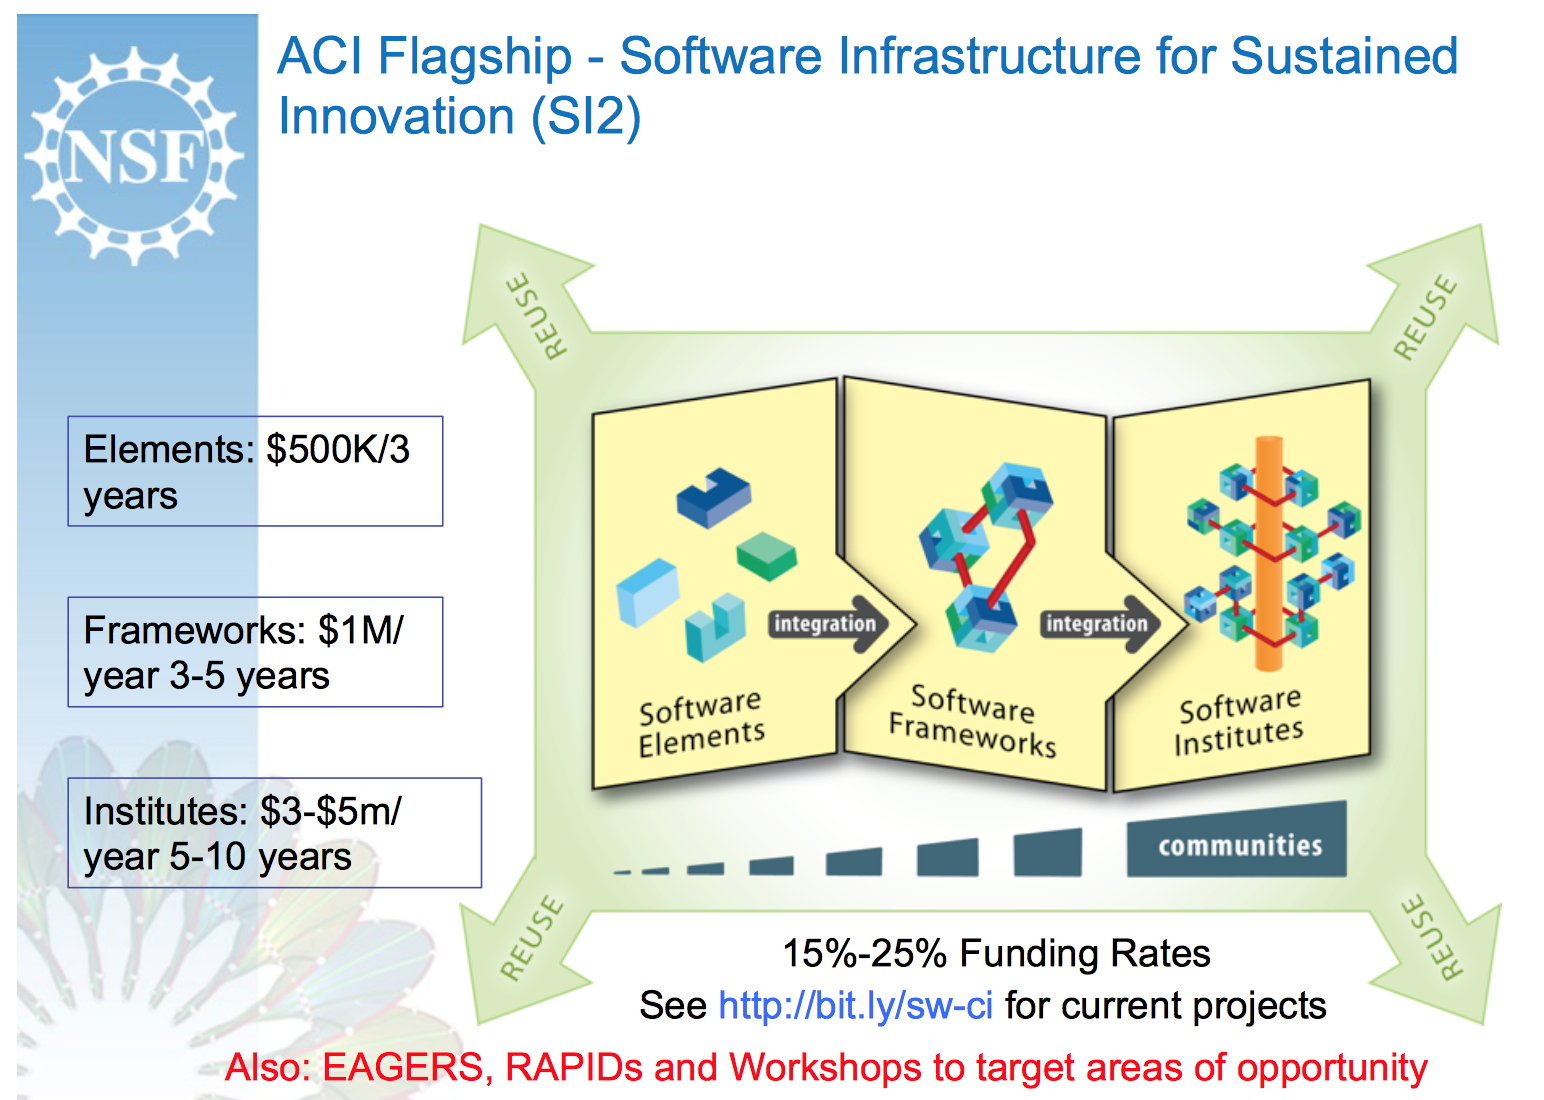
\includegraphics[width=0.75\textwidth]{images/ramnath-si2-pi-meeting-2016.png}
%\caption{}
\label{fig:nsfsi2}
\end{center}
\end{figure}

DIANA/HEP is a ``Software Framework'' (SSI).  The S2I2-HEP project is a planning (conceptualization) ``Software Institute'' award.

\end{frame}



\begin{frame}
\frametitle{NSF SI2 Award Classes}

The NSF SI2 program includes three classes of awards:
\begin{itemize}
\item {\bf Software Elements (SSE)} target small groups that will create and deploy robust software elements for which there is a demonstrated need that will advance one or more significant areas of science and engineering.

\item {\bf Software Frameworks (SSI)} target larger, {\em interdisciplinary} teams organized around the development and application of elements of common software infrastructure aimed at solving common research problems. These awards will result in sustainable community software frameworks serving a diverse community.

\item {\bf Scientific Software Innovation Institutes ($ S^2 I^2 $)} focus on the establishment of long-term hubs of excellence in software infrastructure and technologies, including elements and frameworks, that will serve a {\em research community of substantial size and disciplinary breadth}.
\end{itemize}

\end{frame}




\begin{frame}
\frametitle{The DIANA/HEP project}

\begin{itemize}
\item Data Intensive ANAlysis for High Energy Physics (DIANA/HEP)
\item The primary goal of DIANA/HEP is to develop state-of-the-art tools for experiments which acquire, reduce, and analyze petabytes of data.
\item DIANA is not a piece of software itself, but a collaborative project to improve and extend analysis tools as sustainable infrastructure for the community.
\item Funded by NSF ``Software Infrastructure for Sustained Innovation'' (SI2) program
\item 4-year project, 6-7FTE total
\item Princeton, NYU, UCincinnati, U.Nebraska-Lincoln
\item The PIs are involved in Atlas, CMS and LHCb
\end{itemize}

\end{frame}



\begin{frame}
\frametitle{The DIANA/HEP Project (http://diana-hep.org)}

\begin{figure}[htbp]
\begin{center}
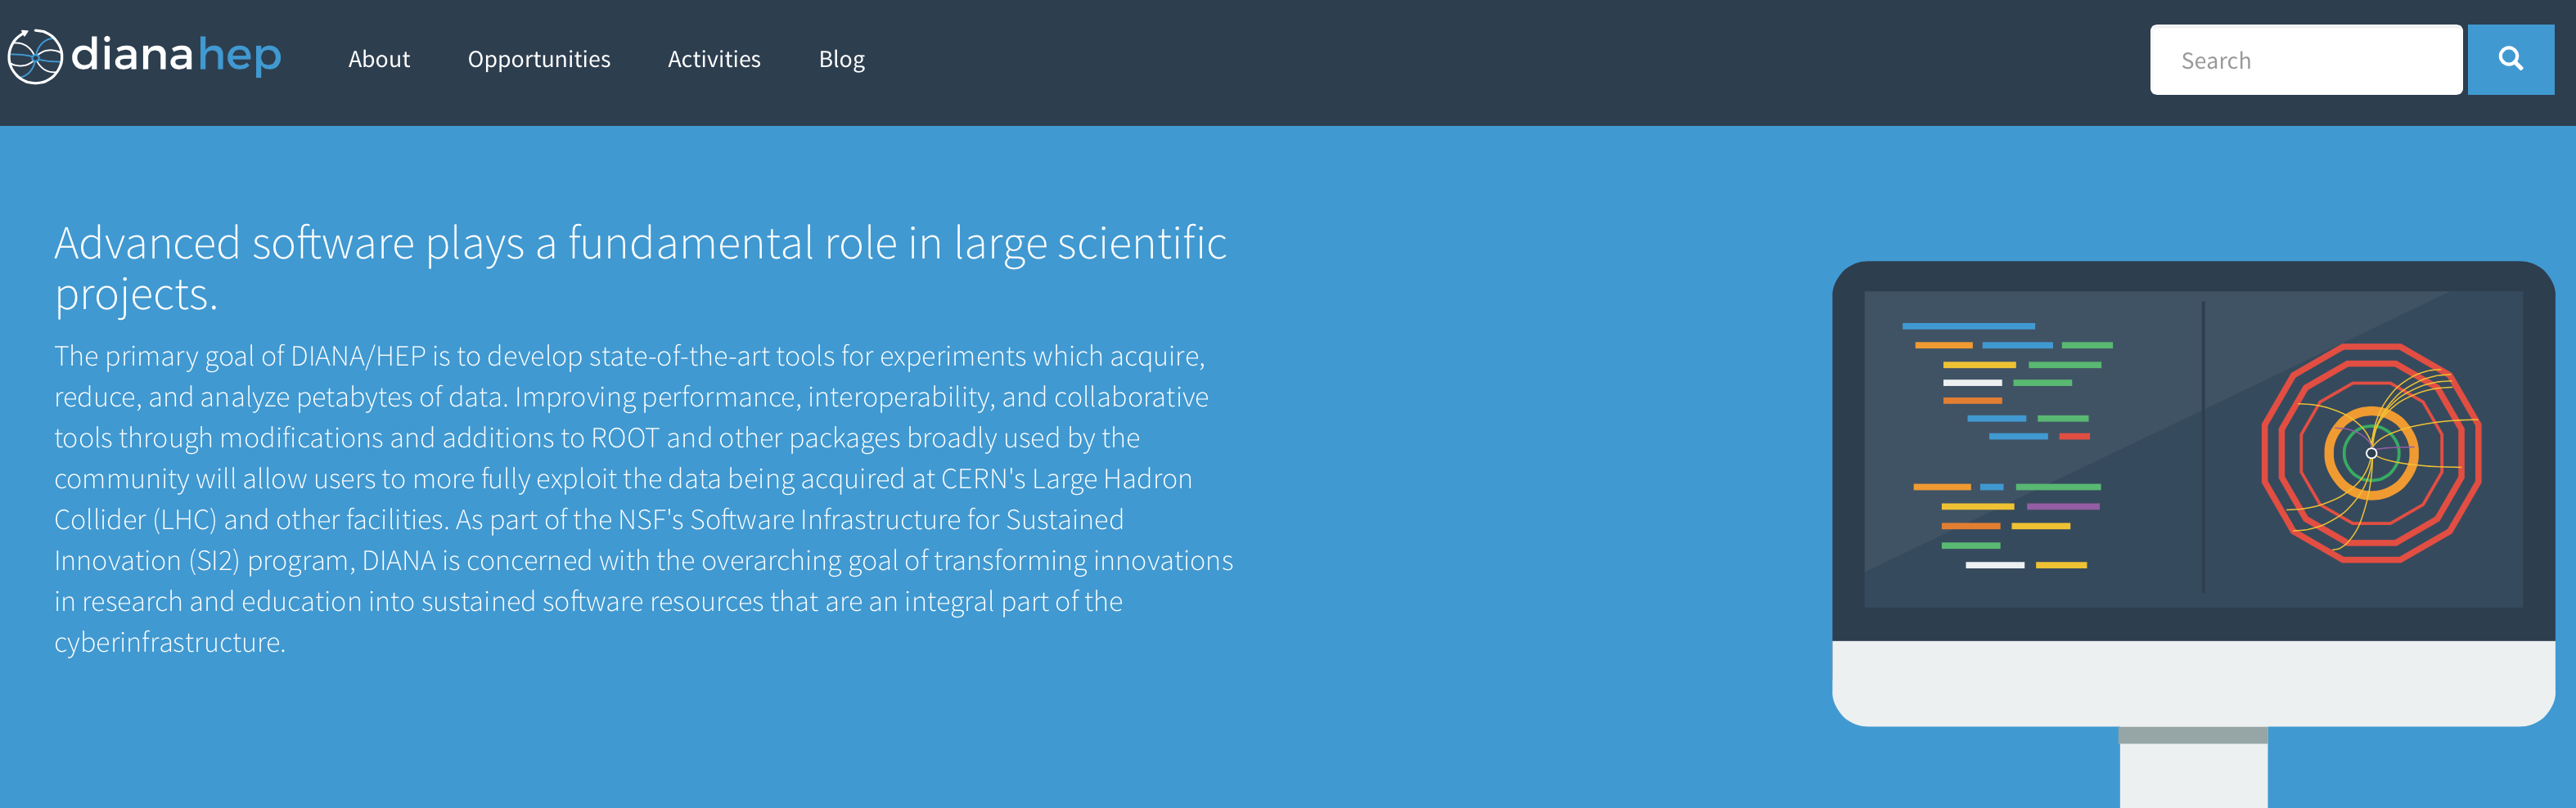
\includegraphics[width=1.0\textwidth]{images/20160610-diana-hep-banner.png}
\end{center}
\end{figure}

\small{The DIANA/HEP project focuses on improving performance, interoperability, and collaborative tools through modifications and additions to ROOT and other packages broadly used by the HEP community.}
\vskip 0.15in
\small{Website: \url{http://diana-hep.org}}
\vskip 0.05in
\small{Google group: \url{https://groups.google.com/forum/\#!forum/diana-hep}}
\vskip 0.05in
\small{Github: \url{https://github.com/diana-hep}}

\end{frame}



\begin{frame}
\frametitle{DIANA/HEP team}

\begin{figure}[htbp]
\begin{center}
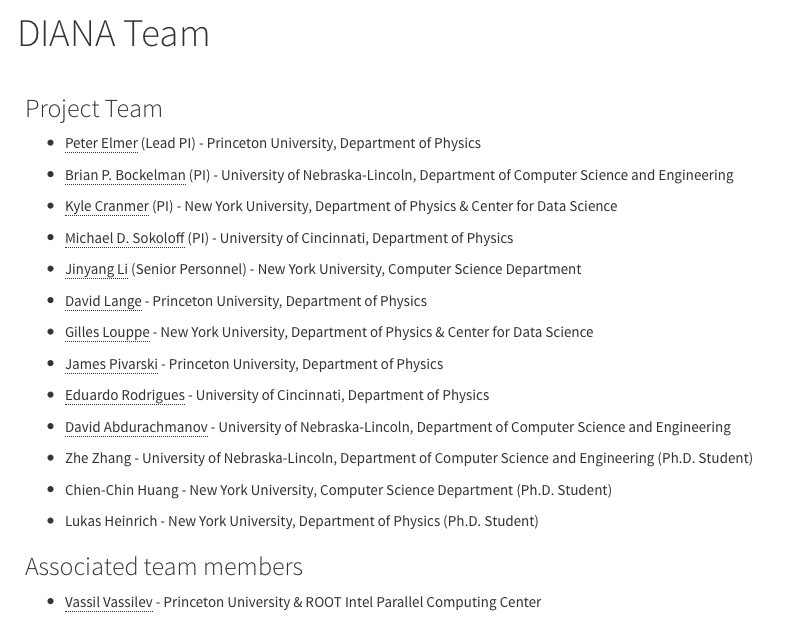
\includegraphics[width=0.9\textwidth]{images/20170110-diana-team.png}
%\caption{}
%\label{fig:example2}
\end{center}
\end{figure}

\end{frame}



\begin{frame}
\frametitle{DIANA/HEP collaborators}

\begin{figure}[htbp]
\begin{center}
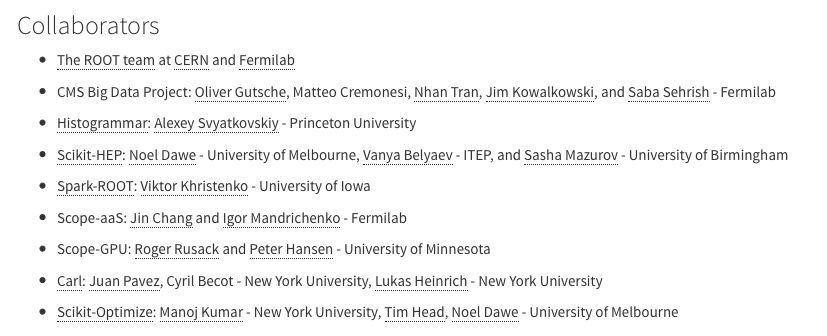
\includegraphics[width=0.9\textwidth]{images/20170110-diana-collaborators.png}
%\caption{}
%\label{fig:example2}
\end{center}
\end{figure}

\end{frame}




\begin{frame}
\frametitle{Example DIANA talks/activities}

\begin{figure}[htbp]
\begin{center}
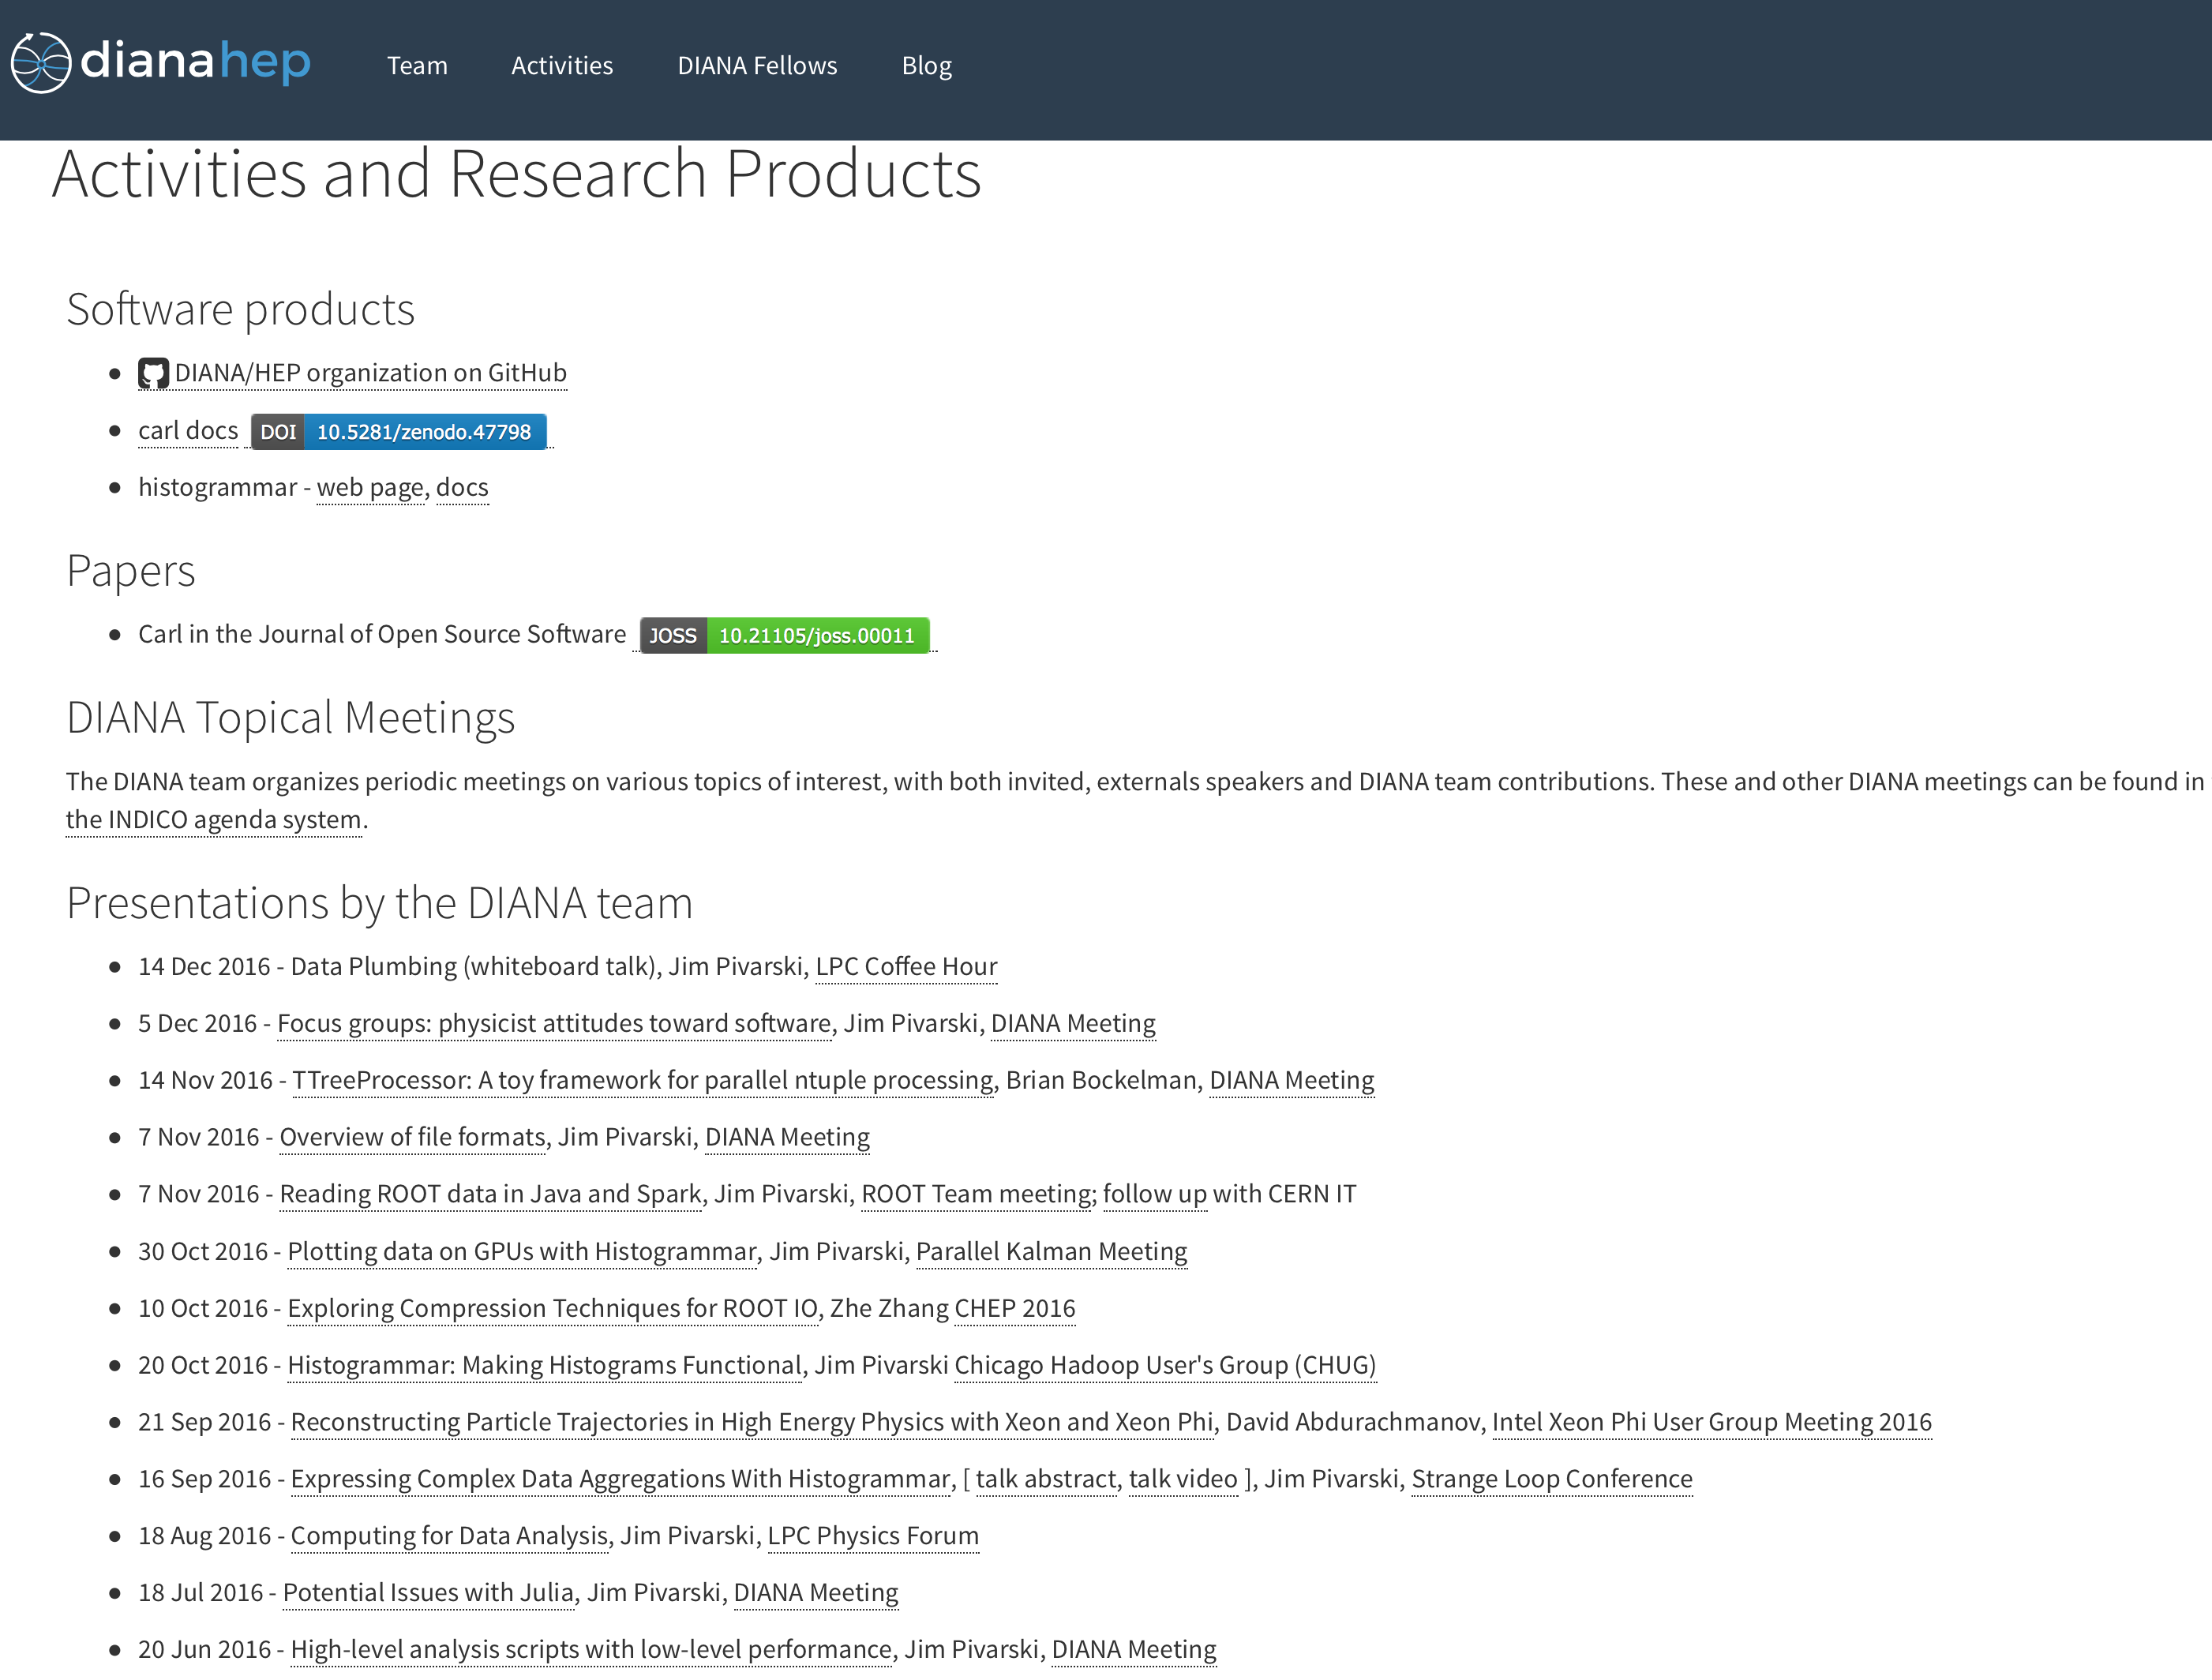
\includegraphics[width=0.8\textwidth]{images/20161213-diana-activities.png}
%\caption{}
%\label{fig:example2}
\end{center}
\end{figure}

%\small{}

\end{frame}



\begin{frame}
\frametitle{DIANA Topical Meetings (\url{https://indico.cern.ch/category/7192/})}

\begin{figure}[htbp]
\begin{center}
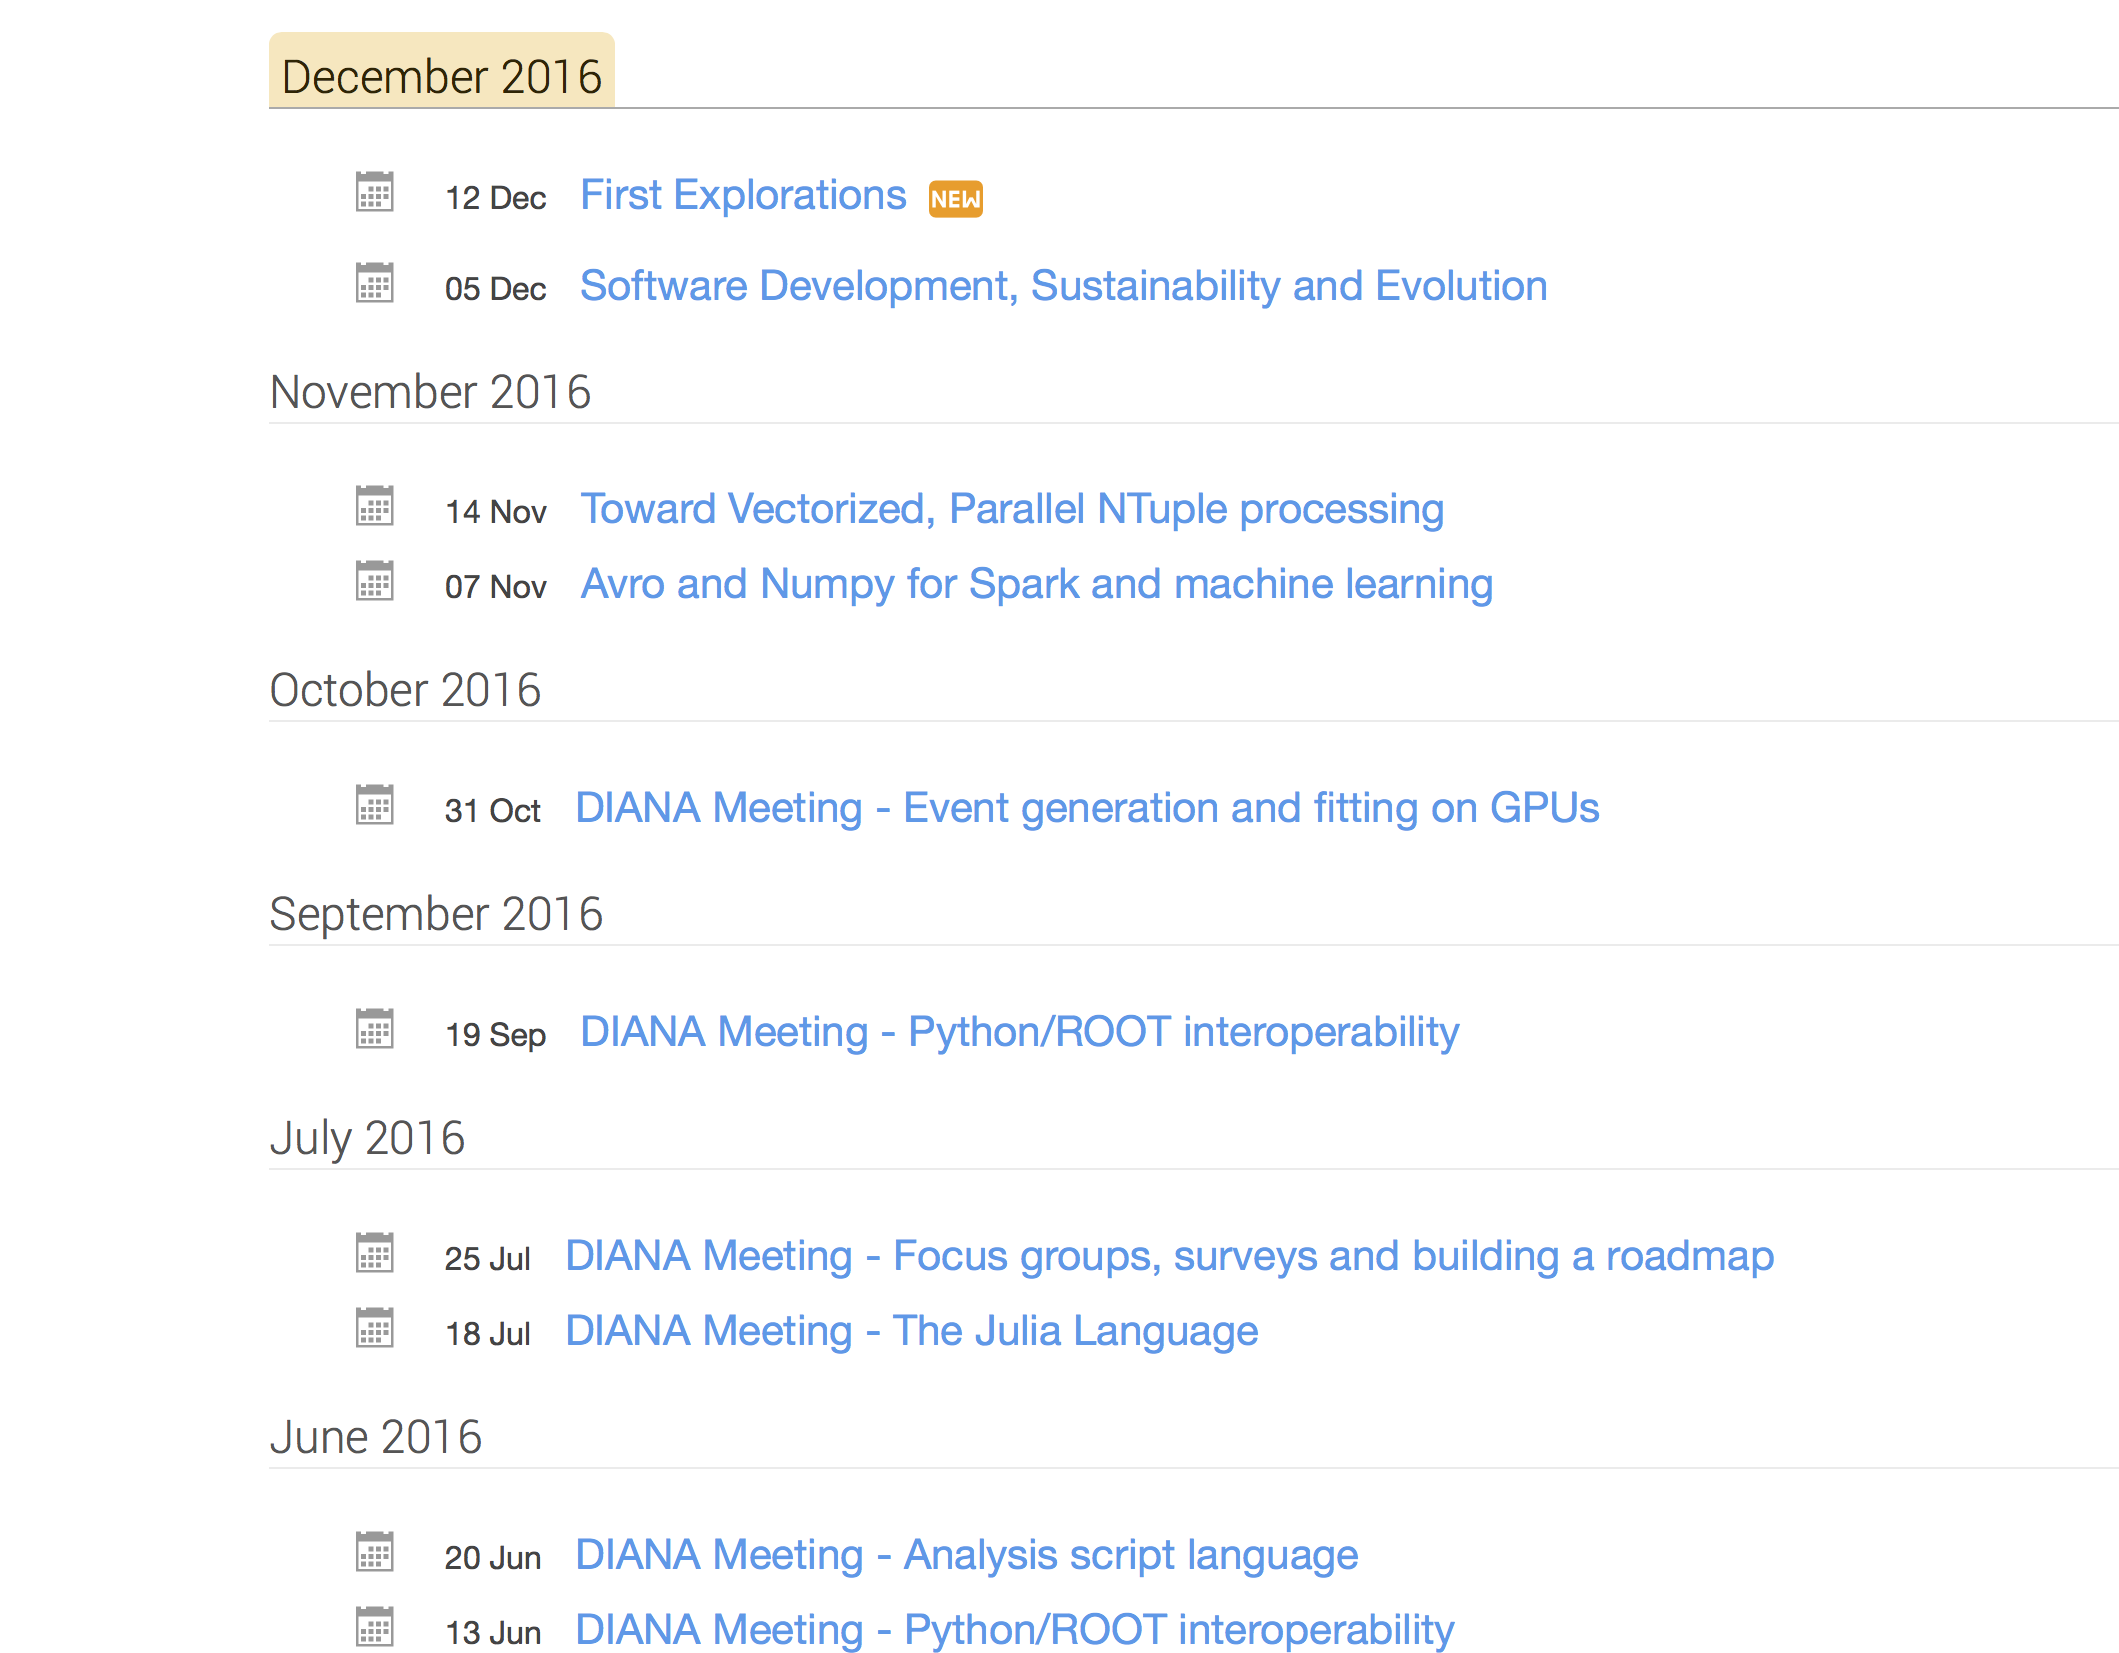
\includegraphics[width=0.8\textwidth]{images/20161213-diana-indico.png}
%\caption{}
%\label{fig:example2}
\end{center}
\end{figure}

%\small{\url{https://indico.cern.ch/category/7192/}}

\end{frame}




\begin{frame}
\frametitle{Upcoming DIANA topical meetings}

\begin{figure}[htbp]
\begin{center}
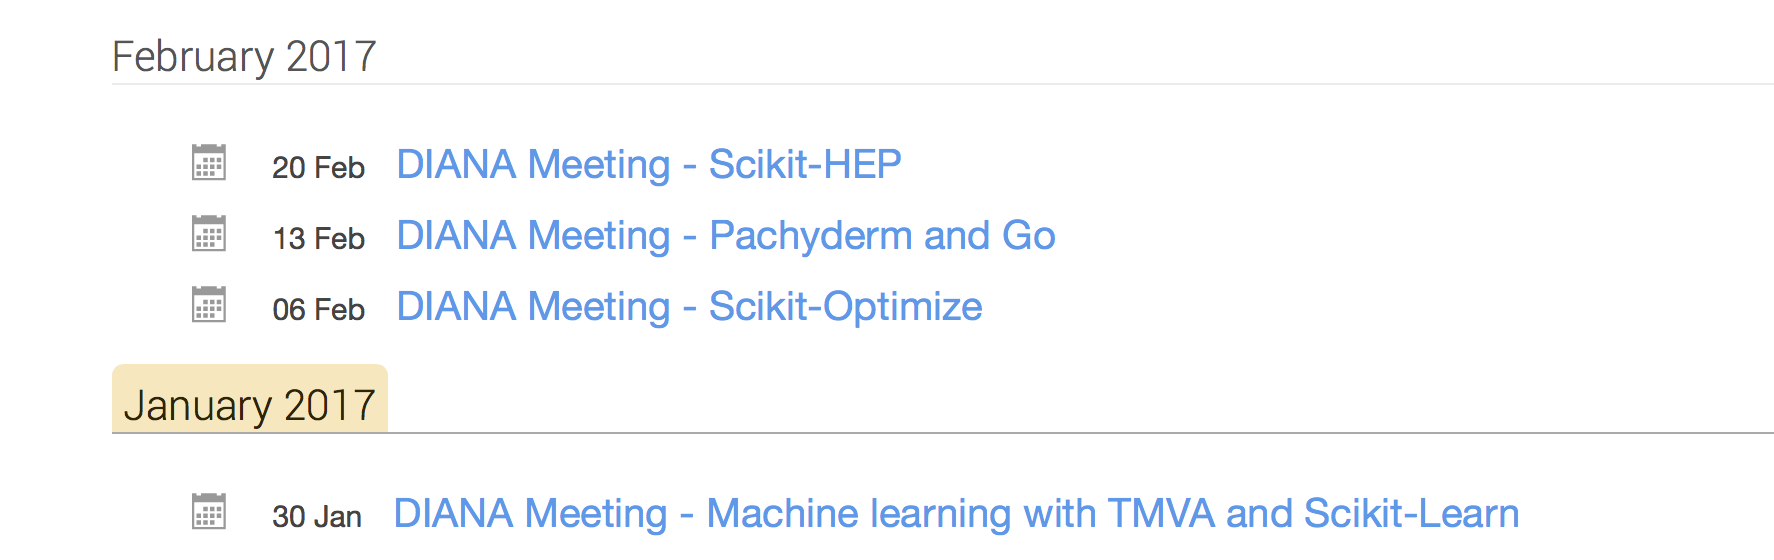
\includegraphics[width=0.8\textwidth]{images/20170110-diana-upcoming.png}
%\caption{}
%\label{fig:example2}
\end{center}
\end{figure}

\end{frame}




\begin{frame}
\frametitle{NSF SI2-S2I2 Software Institute}

NSF SI2-S2I2 includes two subclasses of awards:
\begin{itemize}
\item \underline{Conceptualization Awards} - which are planning awards aimed at organizing an interdisciplinary community and understanding their software requirements and challenges (\$500k, 1-2 years)
\item \underline{Implementation Awards} - which will be made to implement community activities that support software infrastructure, for example, such as those developed by the conceptualization awards (\$3-5M/year, 5 years)
\item NSF funded two software institute implementations last summer (2016):
\item \url{https://www.nsf.gov/news/news_summ.jsp?cntn_id=189347}

\item And they also funded our $ S^2 I^2 $ conceptualization project: 
\begin{itemize}
\item Conceptualization of an $ S^2 I^2 $ Institute for High Energy Physics
\item \url{http://cern.ch/elmer/s2i2-2015-nsf-proposal.pdf}
\end{itemize}
\end{itemize}

\end{frame}



\begin{frame}
\frametitle{S2I2-HEP}
The primary goal of the S2I2-HEP conceptualization project (\url{http://s2i2-hep.org}) is to produce a well-defined strategy for developing the software and computing models for use in high energy physics (HEP), in particular for the experiments collecting the very large data sets anticipated in the ``High-Luminosity Large Hadron Collider'' (HL-LHC) era of the 2020s. \\
\vskip 0.15in
Specifically the S2I2-HEP project will identify potential areas where U.S. university personnel can lead in key areas of software development to help realize the full potential of the HL-LHC program. \\
\vskip 0.15in
However HEP and the LHC are global projects, so no long-term planning exercise can exist in isolation, thus we are also pursuing a wider HEP community roadmap for software and computing in the 2020s.
\end{frame}



\begin{frame}
\frametitle{$ S^2 I^2 $ Conceptualization Awards}

$ S^2 I^2 $ Conceptualization Awards are {\em planning} awards aimed at organizing an interdisciplinary community and understanding their software requirements and challenges. 
Example activities that may be undertaken as part of this award include focused workshops, special sessions at professional meetings, sandpits, focus groups, etc. 
%These awards will typically be 1 year in duration. 
\vskip 0.12in
The product of a conceptualization award will be a {\bf Strategic Plan} for enabling science and education through a sustained software infrastructure that will be freely available to the community. 
\vskip 0.12in
The Strategic Plan resulting from the conceptualization phase is expected to serve as the conceptual design upon which a subsequent $ S^2 I^2 $ Implementation proposal could be based.
\vskip 0.12in
Because an NSF effort cannot stand in isolation to DOE and international efforts, the process we proposed delivers also a broader {\bf Community White Paper}.

\end{frame}




\begin{frame}
\frametitle{HEP Software Foundation (HSF)}

\begin{columns}[T] % align columns

\begin{column}{.75\textwidth}
The HSF (http://hepsoftwarefoundation.org) was created in early 2015 as a means for organizing our community to address the software challenges of future projects such as the HL-HLC. The HSF has the following objectives: 
\end{column}%

\hfill%

\begin{column}{.20\textwidth}
\begin{figure}[htbp]
\begin{center}

\includegraphics[width=1.0\textwidth]{images/hsf_logo_angled.png}
\end{center}
\end{figure}
\end{column}%

\end{columns}

\vskip 0.1in

\begin{itemize}
\item Catalyze new common projects
\item Promote commonality and collaboration in new developments to make the most of limited resources
\item Provide a framework for attracting effort and support to S\&C common projects (new resources!)
\item Provide a structure to set priorities and goals for the work
\end{itemize}

%An initial set of collaborative activities have begun (see recent HSF workshop 
%at LAL-Orsay). 


\end{frame}




\begin{frame}
\frametitle{Recent/Nascent Cross-experiment Collaborations}

\begin{itemize}
\item Experiment frameworks
  \begin{itemize}
  \item Gaudi, FAIRRoot, CMSSW/Art
  \end{itemize}
\item Common Conditions Data Project
  \begin{itemize}
  \item Discussion/cooperation between ATLAS, Belle II, CMS and LHCb
  \end{itemize}
\item Common Software Build and Packaging Tools efforts
  \begin{itemize}
  \item Working group of HSF comparing HEP and non-HEP solutions
  \end{itemize}
\item Cooperation on Reconstruction Software
  \begin{itemize}
  \item ``Connecting the Dots'' tracking workshop, HSF sessions 
  \end{itemize}
\item AIDA2020 (EU funded)
  \begin{itemize}
  \item DD4hep for detector description, PODIO data model library (LCD, FCC, potentially LHCb)
  \end{itemize}
\item DIANA (Data Intensive ANAlysis) (NSF Funded)
  \begin{itemize}
  \item 4-year project on analysis software, including ROOT and its ecosystem
  \end{itemize}
\end{itemize}

\end{frame}



\begin{frame}
\frametitle{Community White Paper (CWP)}

\begin{itemize}
\item The CWP will identify and prioritise the software research and development investments required:
   \begin{itemize} 
   \item to achieve improvements in software efficiency, scalability and performance and to make use of the advances in CPU, storage and network technologies
   \item to enable new approaches to computing and software that could radically extend the physics reach of the detectors
   \item to ensure the long term sustainability of the software through the lifetime of the HL-LHC
   \end{itemize} 
\vskip 0.15in
\item The HSF is engaging the HEP community to produce the CWP via a ``community process''
   \begin{itemize} 
   \item Initiated as an HL-LHC planning process
   \item Aiming for a broader participation (LHC, neutrino program, Belle II, linear collider so far)
   \end{itemize} 
\end{itemize}

\end{frame}




\begin{frame}
\frametitle{Detector Simulation, Triggering, Event Reconstruction and Visualization} 
\scriptsize{
Challenges surrounding high pile-up simulation,
including the CPU resources needed for large statistics samples
needed to compare with data from high trigger rates, high memory
utilization, generation and handling of the large (min-bias) samples
needed to achieve accurate description of high pile-up collision
events, and a flexible simulation strategy capable of a broad
spectrum of precision in the detector response, from ``fast''
(e.g. parametric) simulation optimized for speed to full simulation
in support of precision measurements and new physics searches
(e.g. in subtle effects on event kinematics due to the presence of
virtual particles at high scale).
Software required to emulate upgraded detectors (including the
trigger system) and support determination of their optimal
configuration and calibration. $\bullet$
Software in support of triggering
during the HL-LHC, including algorithms for the High-level Trigger,
online tracking using GPUs and/or FPGAs, trigger steering, event
building, data ``parking'' (for offline trigger decision), and data
flow control systems. $\bullet$ New approaches to event reconstruction, in
which the processing time depends sensitively on instantaneous
luminosity, including advanced algorithms, vectorization, and
execution concurrency and frameworks that exploit many-core
architectures. In particular, charged particle tracking is expected
to dominate the event processing time under high pile-up
conditions. $\bullet$ Visualization tools, not only in support of upgrade
detector configurations and event displays, but also as a research
tool for data analysis, education, and outreach using modern tools
and technologies for 3D rendering, data and geometry description and
cloud environments.
}
\end{frame}



\begin{frame}
\frametitle{Data Access and Management, Workflow and
Resource Management}
\scriptsize{ 
Data handling systems that scale to the Exabyte level during the
HL-LHC era and satisfy the needs of physicists in terms of metadata
and data access, distribution, and replication. Increasing
availability of very high speed networks removes the need for CPU
and data co-location and allows for more extensive use of data
access over the wide-area network (WAN), providing failover
capabilities, global data namespaces, and caching. $\bullet$ Event-based data
streaming as complementary to the more traditional dataset-based or
file-based data access, which is particularly important for
utilizing opportunistic cycles on HPCs, cloud resources, and campus
clusters where job eviction is frequent and stochastic. $\bullet$ Workflow
management systems capable of handling millions of jobs running on a
large number of heterogeneous, distributed computing resources, with
capabilities including whole-node scheduling, checkpointing, job
rebrokering, and volunteer computing. $\bullet$ Systems for measurement and
monitoring of the networking bandwidth and latency between resource
targets and the use of this information in job
brokering. $\bullet$ Software-defined networking technologies which enable
networks to be configurable and schedulable resources for use in the
movement of data.
}

\end{frame}



\begin{frame}
\frametitle{ Physics generators, Data Analysis and Interpretation, Data and Software Preservation}
\scriptsize{ 
There are many theory challenges in the HL-LHC era, among them are
improving the precision of SM calculations, better estimation of
systematic uncertainties, and elucidation of promising new physics
signals for the experiments. Software needed to make connection
between observations and theory include matrix element generators,
calculation of higher-order QCD corrections, electroweak
corrections, parton shower modeling, parton matching schemes, and
soft gluon resummation methods. Physics generators that employ
concurrency and exploit many-core architectures will play an
important role in HL-LHC, as well better sharing of code and
processing between LHC experimenters and phenomenologists. $\bullet$ Data
analysis frameworks that include parallelization, optimized event
I/O, data caching, and WAN-based data access. Analysis software
that employs advanced algorithms and efficiently utilizes many-core
architectures. $\bullet$ Tools and technologies for preservation and reuse of
data and software, preservation and re-interpretation of physics
results, analysis providence and workflow ontologies, analysis
capture, and application packaging for platform abstraction. $\bullet$ Future
software repositories and build platforms that leverage advances in
these areas and improved software modularity and quality control
that will allow a broader community of people to effectively
contribute to software in the HL-LHC era.}

\end{frame}




\begin{frame}
\frametitle{Practicalities: CWP Process}

\begin{itemize}
\item The end goal here is a single (consensus) CWP roadmap for the community. 
\item Finding consensus in a large community is a difficult task: broad participation and visibility/transparency are key elements
\item The process being used largely mirrors that used in the ``decadal survey'' process in high energy physics
\item Working groups self-organize, with encouragement from institutions and projects/experiments/etc.
\item A series of workshops is planned over about 9 months to allow topics to be explored, sometimes overloading CWP discussions onto preexisting meetingd
\item Contributions along the way can come in the form of ``white papers'' by individuals/groups/projects/institutions
\item Based on the ideas emerging from the discusions, workshops and white papers, a consensus CWP document will be written.
\end{itemize}

\end{frame}



\begin{frame}
\frametitle{Practicalities: HSF Google Groups}

The following Google Groups are relevant:

\begin{itemize} 

\item Group for discussion of Community White Paper
  \begin{itemize} 
  \item {\color{blue} \url{https://groups.google.com/forum/\#!forum/hsf-community-white-paper}}
  \end{itemize} 

\item General announcement group for community messages (low traffic)
  \begin{itemize} 
  \item {\color{blue} \url{https://groups.google.com/forum/\#!forum/hep-sw-comp}}
  \end{itemize} 

\item Community Discussion list
  \begin{itemize} 
  \item {\color{blue} \url{https://groups.google.com/forum/\#!forum/hep-sf-forum}}
  \end{itemize} 

\item Specific group for US NSF Software Institute Conceptualization
  \begin{itemize} 
  \item {\color{blue} \url{https://groups.google.com/forum/\#!forum/s2i2-hep}}
  \end{itemize} 

\end{itemize} 

\end{frame}



\begin{frame}
\frametitle{Practicalities: Possible Working Groups}
\begin{table}[h!]
\tiny
\centering
\label{tab:table1}
\begin{tabular}{|l|l|}
\hline
Detector Simulation & full and fast simulations, hi-pileup environments \\ \hline

Triggering & algorithms, GPUs and/or FPGAs \\ \hline

Event Reconstruction & new approaches to event reconstruction \\ \hline

Visualization & tools for data analysis, education, and outreach \\ \hline

Data Access and Management & scaling to the exabyte level \\ \hline

Workflow and Resource Management & millions of jobs in heterogenous systems \\ \hline

Physics generators & better models, better precision, code optimisations \\ \hline

Data Analysis and Interpretation & efficient use of many-core, modern techniques \\ \hline

Data and Software Preservation & preservation and reuse of data and software \\ \hline

Software Development, Deployment & \\
and Validation/Verification & improved modularity and quality, contribution \\ \hline

Computing Models, Facilities, & \\
Distributed Computing & range of possible models, costing\\ \hline

Various Aspects of Technical Evolution & \\ 
(Software Tools, Hardware) &  \\ \hline

Security and Access Control & \\ \hline

Careers, Staffing and Training & perhaps in a separate concurrent white paper \\ \hline

Machine Learning & \\ \hline

Conditions Database & \\ \hline

Event Processing Frameworks & \\ \hline
\end{tabular}
\end{table}

\begin{center}
\small{More details in links at \color{blue} {\url{http://hepsoftwarefoundation.org/cwp.html}}}
\end{center}

\end{frame}




\begin{frame}
\frametitle{HSF Community White Paper Workshop at SDSC}

\begin{itemize}
\item The kick-off workshop for the HSF CWP process will be on 23-26 January 2017 at SDSC/UCSD
\item \url{http://indico.cern.ch/event/570249/}
\item People from many HEP experiments (LHC and beyond)
\item A key element in the ``community process'' to form a consensus
\item We are looking for opportunities to introduce new ideas into the HEP discussions
\item An early strawman agenda is posted (next slides, but evolving quickly so online version has the latest)
\item Registration is open (see URL above)
\end{itemize}

\end{frame}




\begin{frame}
\frametitle{Possible routes to a ``Software Upgrade''}

\begin{itemize}
\item If we are aiming at a larger ``software upgrade'' project towards the HL-LHC, an additional ingredient is to find (or liberate/reallocate) the resources to realize this roadmap. 
\item We need both initial exploratory R\&D and eventual development projects!
\item In the US, both the NSF and the DOE have at least the notion of eventual resources and/or organization for new common projects in HEP (NSF: SI2, DOE: HEP CCE)
  \begin{itemize}
   \item The US NSF has funded a ``conceptualization'' (planning) project with a possible path towards a ``Software Institute'' (\url{http://s2i2-hep.org})
   \item The US DOE has seeded the ``Center for Computing Excellence'' with some initial resources. (\url{http://hepcce.org})
  \end{itemize}
\item We hope that a clear community roadmap will bring these and other partners together for an HL-LHC software upgrade.
\end{itemize}

\end{frame}




\begin{frame}
\frametitle{S2I2-HEP (Success-oriented) timeline}

\begin{figure}[htbp]
\begin{center}
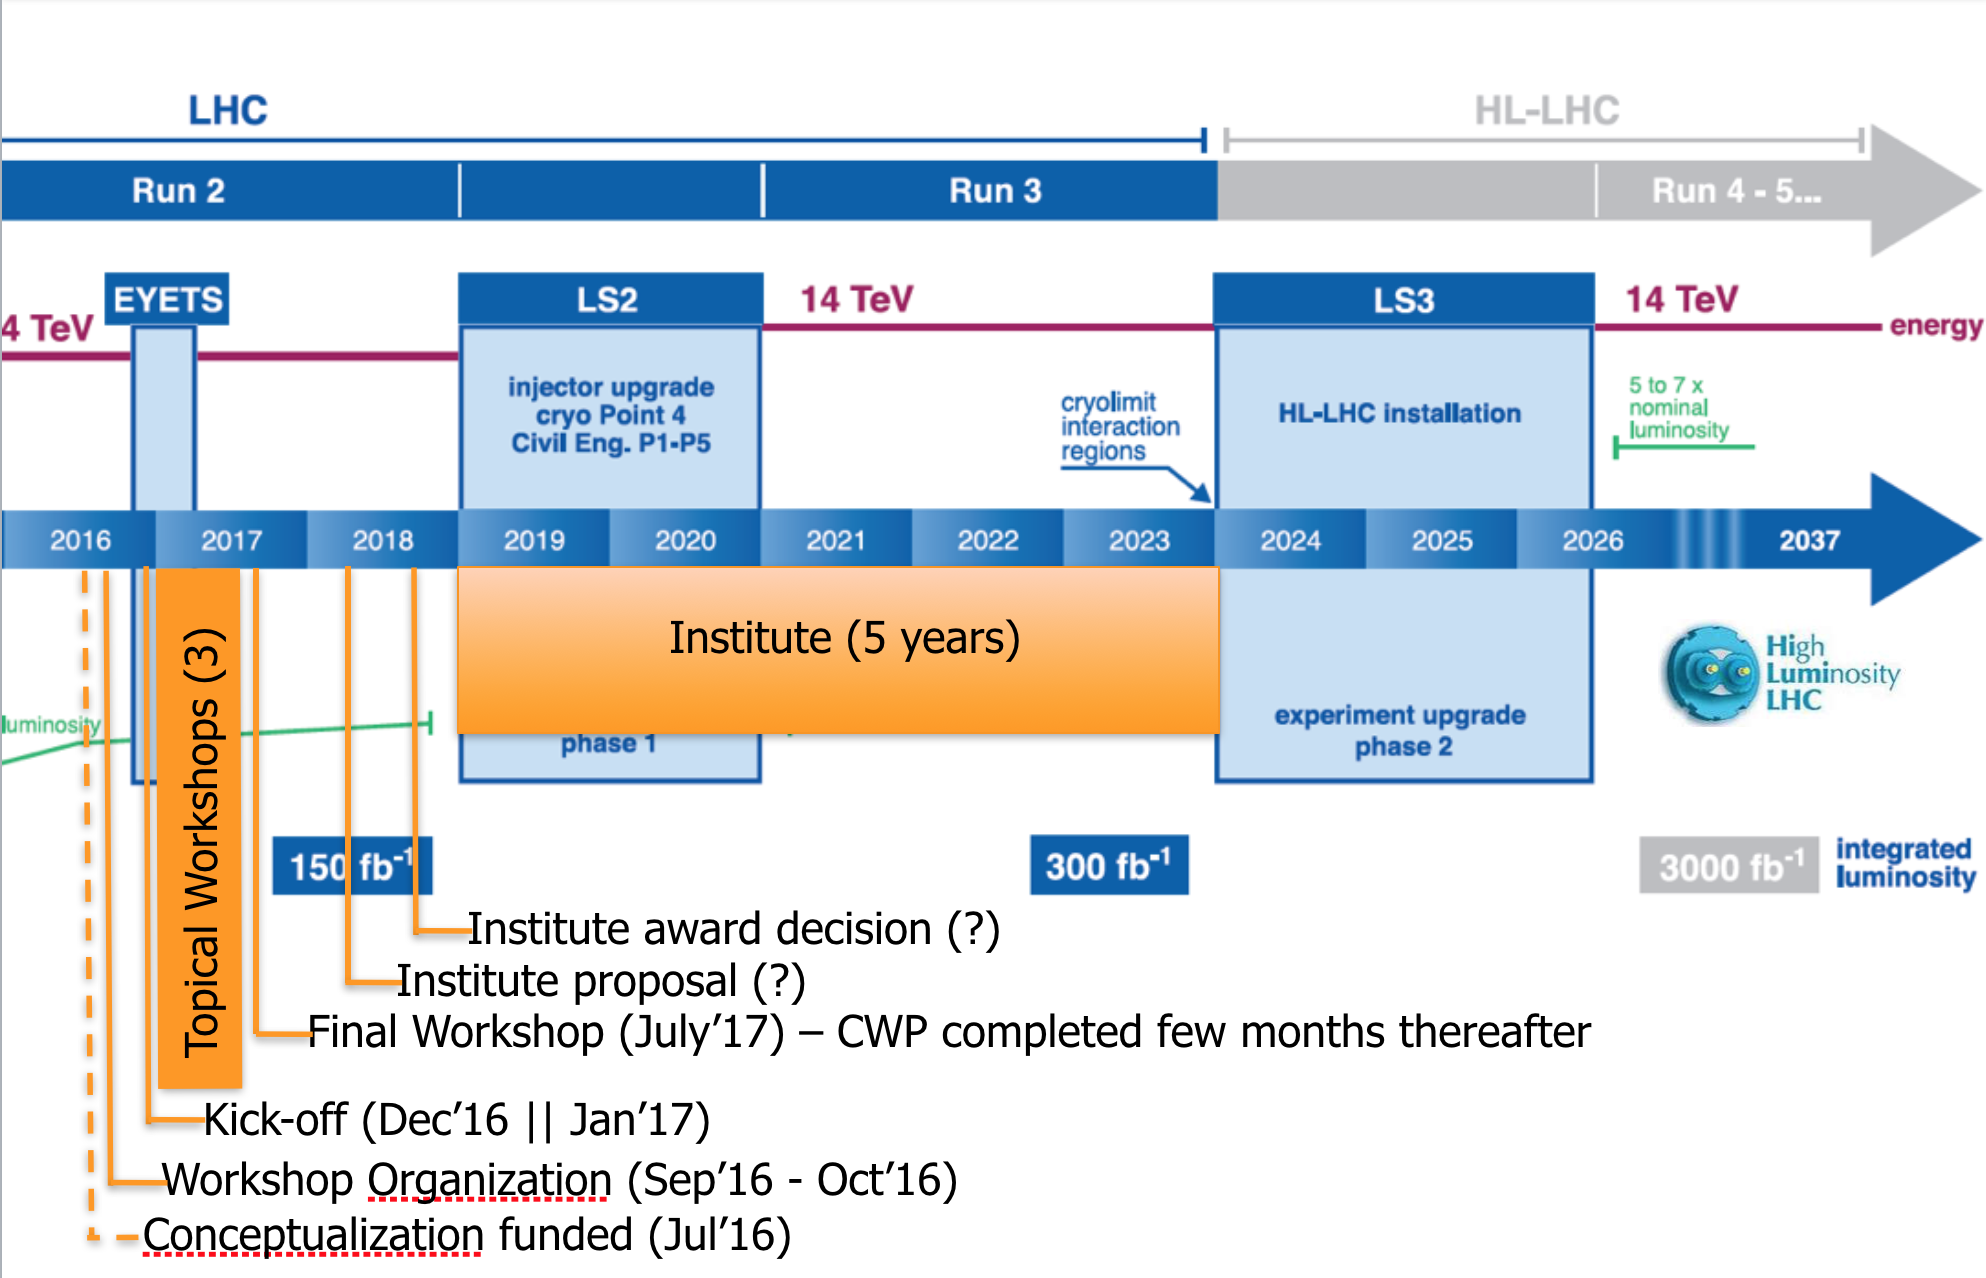
\includegraphics[width=1.0\textwidth]{images/s2i2-hep-timeline.png}
%\caption{}
%\label{fig:example2}
\end{center}
\end{figure}

%\small{Example Text}

\end{frame}




\begin{frame}
\frametitle{Monday Plenary Agenda (evolving)}

\begin{figure}[htbp]
\begin{center}
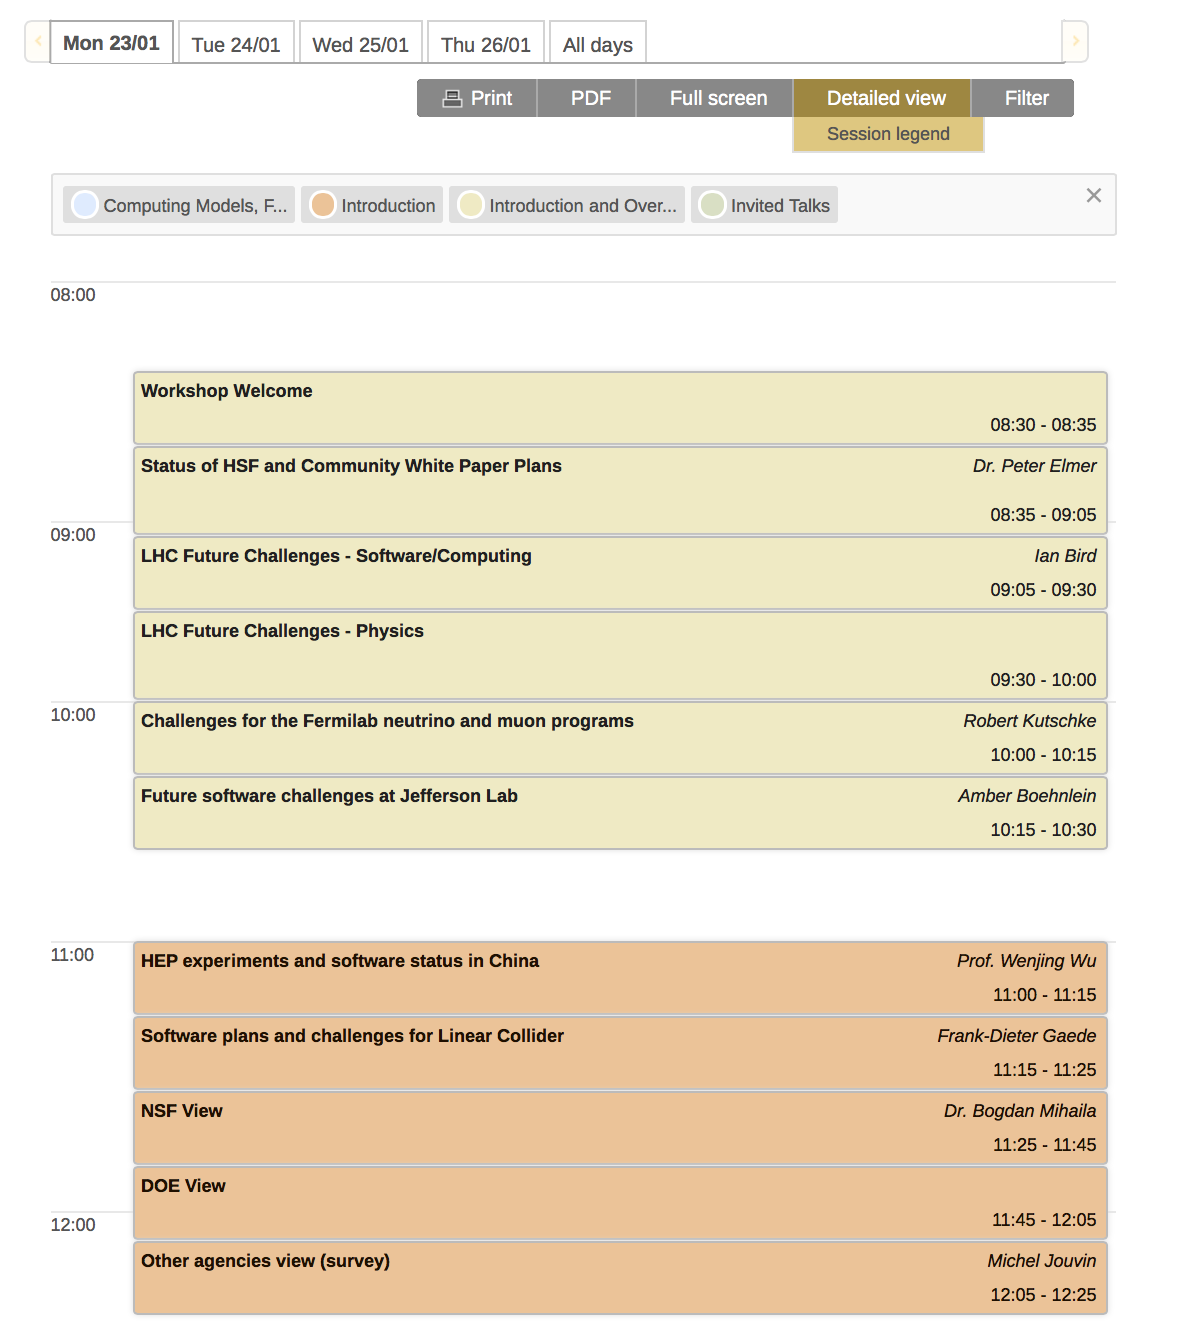
\includegraphics[width=0.7\textwidth]{images/20170110-HSF-SDSC-Workshop-1.png}
%\caption{}
%\label{fig:example2}
\end{center}
\end{figure}

\small{Example Text}

\end{frame}



\begin{frame}
\frametitle{Wednesday Parallel Agenda (evolving)}

\begin{figure}[htbp]
\begin{center}
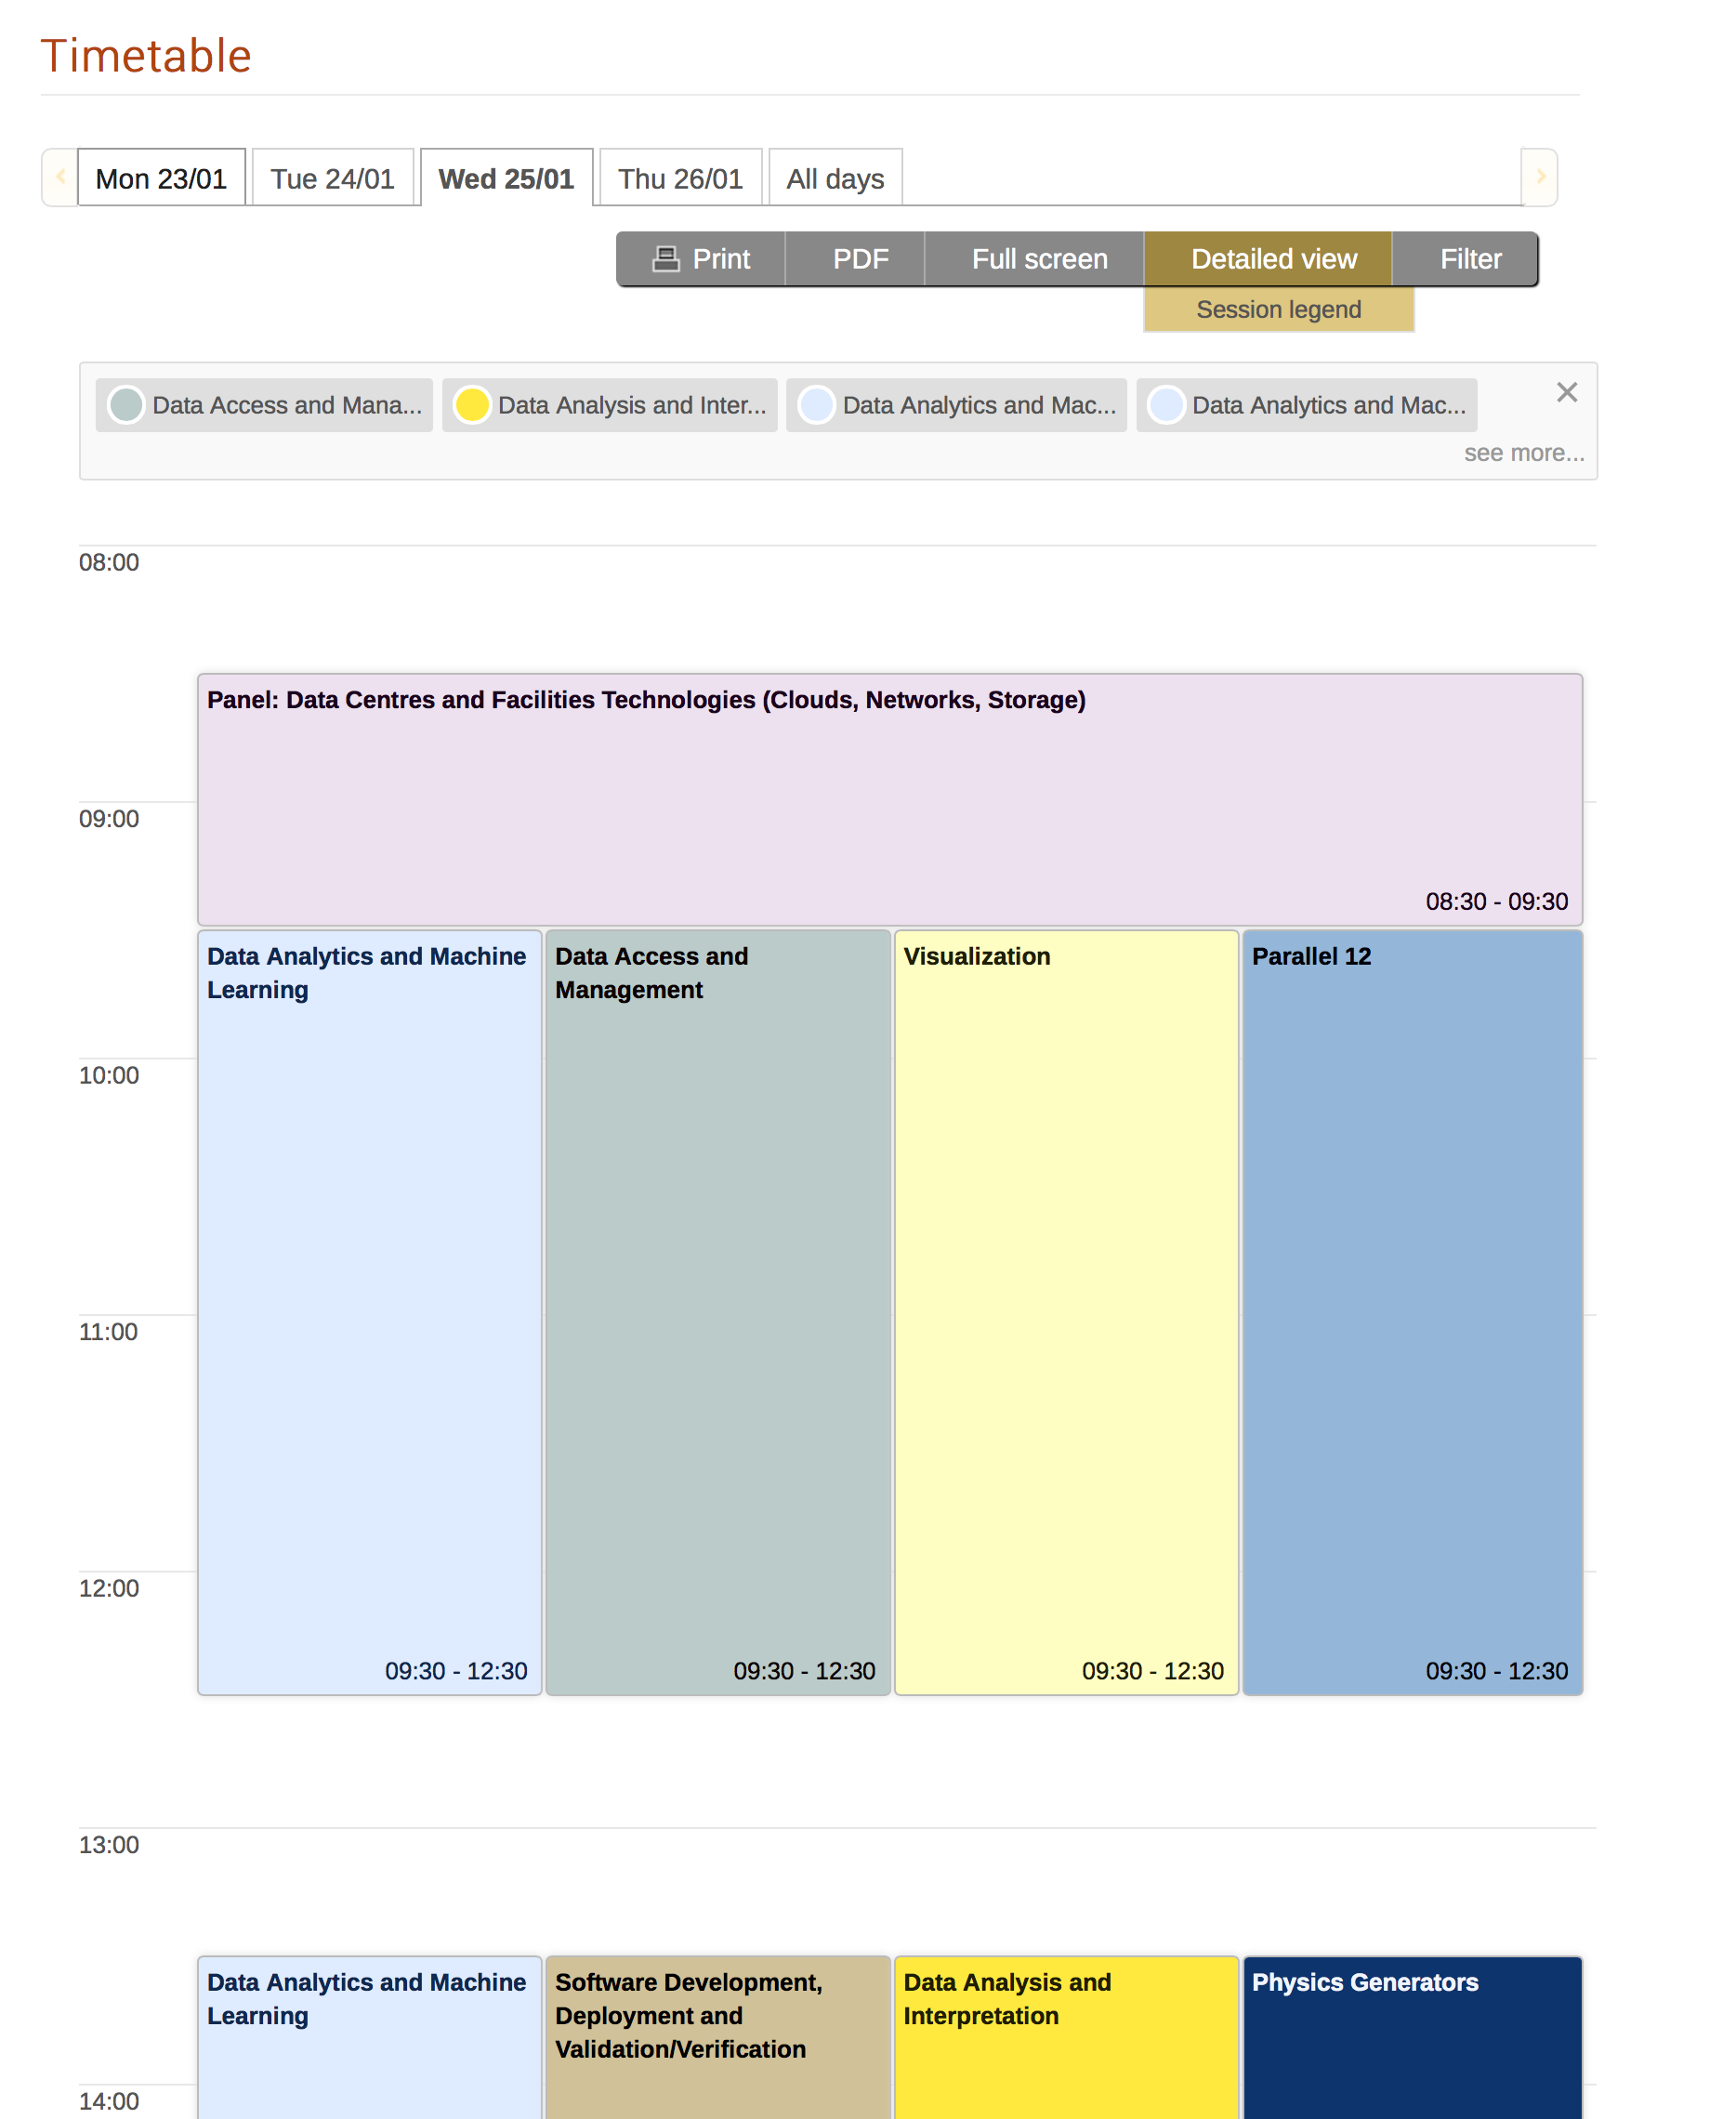
\includegraphics[width=0.7\textwidth]{images/20161214-HSF-SDSC-Workshop-2.png}
%\caption{}
%\label{fig:example2}
\end{center}
\end{figure}

\small{Example Text}

\end{frame}




%%%%%%


\begin{frame}
\frametitle{Practicalities: Contributing White Papers}

\begin{itemize}
\item The end goal here is a single CWP roadmap for the community. 
\item Along the way people are encouraged to put ideas on the table by submitting topical white papers. 
\item \url{http://hepsoftwarefoundation.org/cwp-whitepapers.html}
\item Note in particular the request for contributed white papers on ``Computing Models, Facilities and Distributed Computing''
by 15 January, 2017
\item \url{http://hepsoftwarefoundation.org/cwp/CWPWhitePaperSolicitation.pdf}
\item Existing public documents are also something we will build upon, e.g. the Snowmass Computing documents, the DOE HEP-CCE documents, the WLCG Run2 Computing Model Update, the CERN Openlab whitepaper, etc. Feel free to send links to these, too.
\end{itemize}

\end{frame}




\begin{frame}
\frametitle{Summary}

\begin{itemize}
\item We have a significant investment in software, it embodies the core of our intellectual property and the real cyberinfrastructure.
\item Significant challenges of scale, performance, technology and long term sustainability exist as we face the projects of the 2020s.
\item DIANA/HEP is a pilot project to understand how to build sustainable software and software communities
\item The LHC and wider HEP communities are also executing a planning process for medium/long term software and computing R\&D
\item The process should produce the ``Community White Paper'', a roadmap for HEP Software and Computing for the 2020s
\item In parallel we would like to investigate funding and collaboration possibilities for eventual projects and activities
\item Please consider participating in the CWP process, the WGs and the workshops (beginning with the HSF workshop SDSC/UCSD in January 2017) and to put forward ideas in white papers
\end{itemize}

\end{frame}



%\begin{frame}
\frametitle{HEP Software Ecosystem}

\begin{figure}[htbp]
\begin{center}
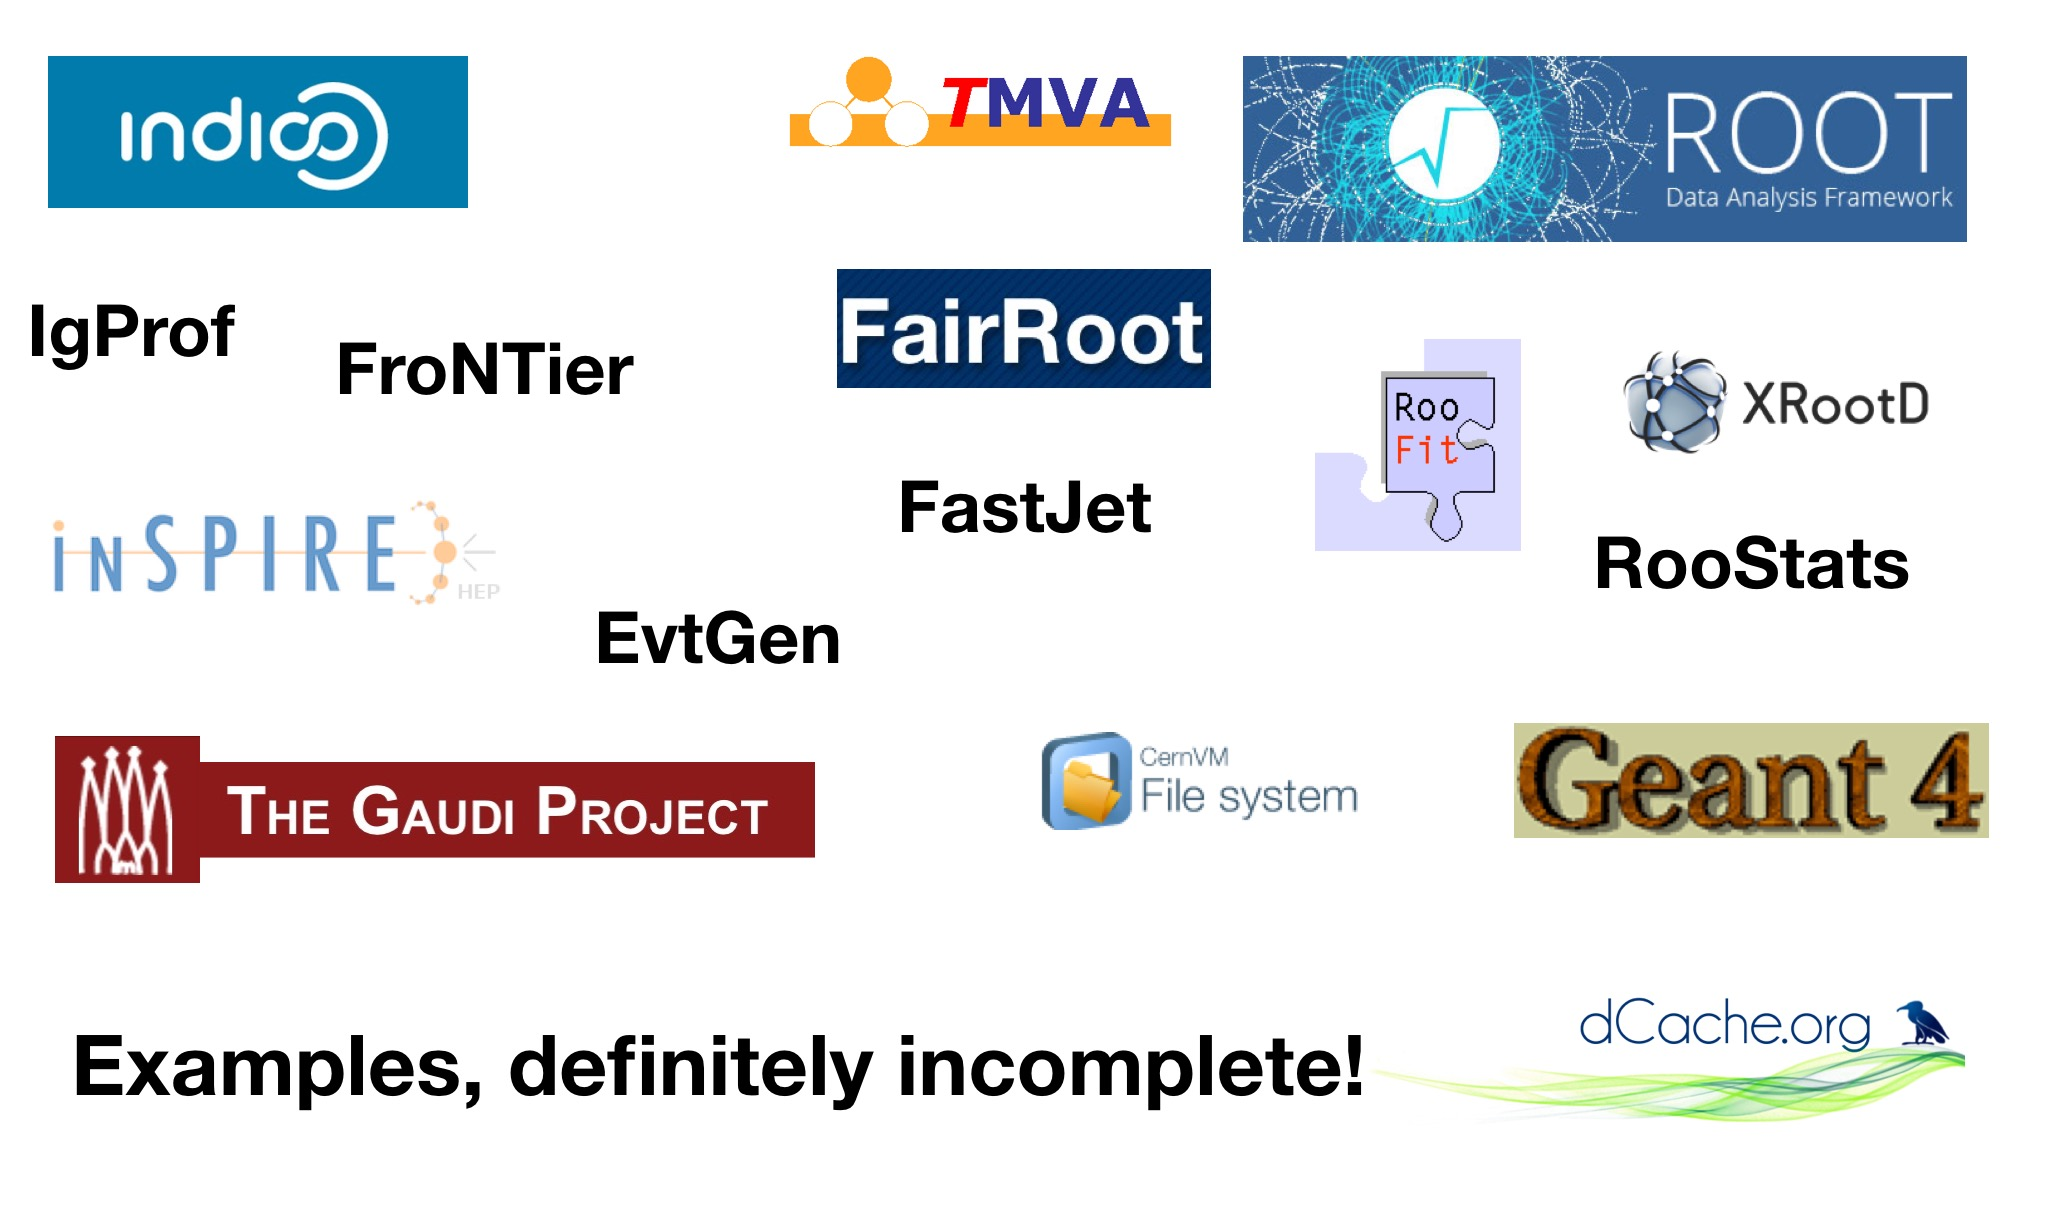
\includegraphics[width=0.9\textwidth]{images/hep-software-ecosystem.jpg}
\end{center}
\end{figure}

\end{frame}




\end{document}


